% !TeX program = pdflatex
% Overleaf: main.tex is the main document; compiler = pdfLaTeX.
% The three supplied vector figure plates are included at their native large-format size.
% Editable plate source: figure_plates.tex. Recompile that file only when changing figures.
\documentclass[11pt,a4paper]{article}
\usepackage[T1]{fontenc}
\usepackage[utf8]{inputenc}
\usepackage[english]{babel}
\usepackage[a4paper,margin=25mm,headheight=14pt]{geometry}
\usepackage{amsmath,amsthm}
\usepackage{newtxtext,newtxmath}
\usepackage{microtype,bm}
\usepackage{siunitx}
\sisetup{group-separator={,},group-minimum-digits=4}
\usepackage{graphicx,booktabs,tabularx,array,longtable,multirow}
\usepackage{xcolor}
\definecolor{forest}{HTML}{1EA23C}
\definecolor{forestink}{HTML}{186D30}
\definecolor{sourceblue}{HTML}{006786}
\definecolor{papergray}{HTML}{F3F2F2}
\usepackage[numbers,sort&compress]{natbib}
\renewcommand{\bibfont}{\small}
\setlength{\bibsep}{4pt}
\usepackage{url}
\usepackage[hyphens]{xurl}
\usepackage{caption}
\captionsetup{font=small,labelfont=bf,justification=justified,singlelinecheck=false}
\usepackage{enumitem}
\usepackage{fancyhdr}
\usepackage{titlesec}
\usepackage{pdfpages}
\usepackage{hyperref}
\hypersetup{colorlinks=true,linkcolor=sourceblue,citecolor=sourceblue,urlcolor=sourceblue,
 pdftitle={From tropical forest-carbon measurement to annual carbon accounts},
 pdfauthor={Henry Arellano-Peña},pdfsubject={Methodology: independent stand-carbon reconstruction and annual-transfer analysis},
 pdfkeywords={pantropical carbon, measurement protocol, basal area, woody volume, material properties, calibration, stock-to-flux transfer, source accounting}}
\usepackage[nameinlink,capitalise]{cleveref}
\pagestyle{fancy}
\fancyhf{}
\fancyhead[L]{\small\itshape Forest-carbon measurement and annual accounts}
\fancyhead[R]{\small Arellano-Pe\~na}
\fancyfoot[C]{\thepage}
\renewcommand{\headrulewidth}{0.3pt}
\titleformat{\section}{\large\bfseries\color{sourceblue}}{\thesection}{0.65em}{}
\titleformat{\subsection}{\normalsize\bfseries}{\thesubsection}{0.65em}{}
\titlespacing*{\section}{0pt}{2.2ex plus .7ex minus .3ex}{1.2ex}
\titlespacing*{\subsection}{0pt}{1.6ex plus .5ex minus .2ex}{.8ex}
\setlength{\parindent}{1.25em}
\setlength{\parskip}{.22em}
\linespread{1.08}
\setlength{\emergencystretch}{2em}
\setcounter{secnumdepth}{3}
\newcolumntype{Y}{>{\raggedright\arraybackslash}X}
\newcommand{\COtwo}{\ensuremath{\mathrm{CO}_2}}
\newcommand{\COtwoe}{\ensuremath{\mathrm{CO}_2\mathrm{e}}}
\newcommand{\GtC}{\ensuremath{\mathrm{GtC}}}
\newcommand{\PgC}{\ensuremath{\mathrm{PgC}}}
\newcommand{\E}{\mathbb{E}}
\DeclareMathOperator{\Cov}{Cov}
\DeclareMathOperator{\Var}{Var}
\DeclareMathOperator{\MSE}{MSE}
\DeclareMathOperator{\rank}{rank}
\DeclareMathOperator{\diag}{diag}
\newtheorem{proposition}{Proposition}[section]
\newtheorem{corollary}[proposition]{Corollary}
\theoremstyle{remark}
\newtheorem{remark}[proposition]{Remark}
\title{\vspace{-1.2em}\textbf{From tropical forest-carbon measurement to annual carbon accounts}\\[.5em]
\large A measurement protocol linking stand structure, carbon calibration and annual accounts}
\author{Henry Arellano-Pe\~na\\[.3em]\small NEBIOT S.A.S., Bogot\'a, Colombia\\[.2em]\small Correspondence: \href{mailto:harellano@unal.edu.co}{harellano@unal.edu.co}}
\date{17 September 2026}
\newcommand{\MeanCarbon}{258.65}
\newcommand{\MeanBiomass}{550.32}
\newcommand{\HighBiomass}{1004.66}
\newcommand{\FeldDensity}{170.97}
\newcommand{\MixedDensityRatio}{1.513}
\newcommand{\HighDensityRatio}{2.762}
\newcommand{\HighStockRatio}{1.988}
\newcommand{\HighAreaRatio}{0.720}
\newcommand{\TestAssertions}{257167}
\newcommand{\TestCases}{1000}
\newcommand{\ExtendedCases}{20000}

\begin{document}
\maketitle
\thispagestyle{empty}
\begin{abstract}
\textbf{Background.} We specify a measurement protocol for testing mapped forest carbon against independently reconstructed material and propagating calibration into annual accounts.

\textbf{Results.} The protocol retains disjoint organ volumes, measured tissue properties and area-weighted plot products. Class 5 of the published 723.97\,PgC pantropical estimate has a printed mean of 531.05 and a stock--area ratio of 536.33\,MgC\,ha$^{-1}$. Illustrative carbon fraction 0.47 and basic density 0.60\,Mg\,m$^{-3}$\ imply about 1,900\,m$^3$ of woody material per hectare. The class edge of 478\,MgC\,ha$^{-1}$\ gives a conditional mapped-cell requirement near 1,700\,m$^3$\,ha$^{-1}$. Five explanations are evaluated: volume, material properties, separately measured compartments, spatial selection and upward bias in the mapped target. Harvest-component evidence constrains foliage as a gap-filling explanation; the protocol specifies held-out, spatially blocked tests to distinguish extrapolation and predictor-resolution failures from structural differences. A published C\'ordoba community supports a reproducible aggregate-data audit but lacks independent organ volumes and matched map values needed for a geometric residual. Direct interval membership corrects two printed class assignments without altering stocks. Exact stock-to-flux and paired-account identities retain disturbance history, regrowth and finite census increments.

\textbf{Conclusions.} The procedure permits corroboration, downward revision or upward revision of a mapped target under explicit measurement and selection criteria, with unresolved comparisons reported separately. The published pantropical value, Australian-tropics exclusion and nominal 2007--2008 epoch are retained as source attributes, not acceptance constraints. A representative empirical class-5 test remains outstanding.
\end{abstract}
\noindent\textbf{Keywords:} pantropical carbon; stand structure; basal area; woody volume; tissue carbon; physical closure; allometric bias; stock-to-flux transfer; source--sink attribution.

\section{Introduction}
A forest-carbon estimate implies a physical arrangement of material: a population of stems and organs, their solid volumes, and the carbon contained in that material. Those quantities provide a forward measurement test distinct from agreement with another biomass predictor. The subsequent atmospheric consequence depends on how that measured carbon enters sources and removals. A positive net source missing from an account leaves actual accumulation above the account's reconstruction unless changes in other terms offset it; release histories determine its timing. The scientific task is therefore to connect measurable stand structure to spatially integrated carbon and then to annual exchange.

The historical forest-carbon reassessment \citep{Arellano2016} motivated two principal accounting interpretations---an underestimated total and a larger contribution assigned to forest loss within a retained total---together with joint source--sink reassessment when several components are uncertain. The subsequent Amazon essay developed the broader interpretation \citep{Arellano2021}. The scientific question is not simply whether a larger forest numerator changes a pie chart. It is whether independently supported biological recalibration changes the physical flows, the accounting allocation, or both.

The published 723.97\,PgC estimate provides a concrete application of this sequence: it represents aboveground carbon in a mapped pantropical domain excluding the Australian tropics, with nominal map epoch 2007--2008 \citep[pp.~23--24]{Arellano2016}. Class 5 alone assigns 285.03\,PgC to 531.45 million hectares. The resulting density defines a quantitative structural target. A measurement-based assessment asks whether independently characterized stand geometry and material properties reproduce that target over representative strata. Architectural and allometric products are assessed by the evidence in their measurement chains and by matched spatial and pool definitions. Contemporary reconstruction and calibration studies supply geographically specific evidence for these comparisons \citep{Gonzalez2018,Momo2018,Demol2024,Huertas2025}.

This article specifies a measurement-to-accounting protocol. Independently obtained geometry and tissue properties generate plot-level carbon, representative spatial weighting generates a class mean, and calibrated disturbance and growth operators generate annual sources and removals. A worked application quantifies the material requirement and comparison gap for class 5 of the published pantropical estimate. The published-table correction supports provenance, while the transfer identities specify operational consequences. Detailed census derivations and the historical emissions-percentage reconstruction are supplied in appendices; they support the protocol rather than constitute an independent inventory.

The figures connect measurement, mapping and accounting. Figures~\ref{fig:reported} and \ref{fig:reinterpretation} adapt the WRI/Ecofys sector--activity--gas organization \citep{WRI2005,Ecofys2013}; their widths are schematic. Figure~\ref{fig:physicalclosure} states the physical class-5 target and the measured inputs required to test it. The pantropical stock, worldwide geographic extension and annual source allocation are separate quantities throughout.

\begin{center}
\fcolorbox{sourceblue}{papergray}{\begin{minipage}{.94\textwidth}\small
\textbf{Research contribution and evidence status.} The study supplies exact stand-closure and annual-transfer identities, a uniquely resolved table assignment within fixed intervals, and reproducible source comparisons. The 723.97\,PgC mapped pantropical estimate retains its published value, Australian-tropics exclusion and nominal 2007--2008 epoch. Geometry-derived targets are conditional requirements, not recovered field observations. Empirical evaluation can corroborate the target or identify its overestimation or underestimation, with threshold-overlapping comparisons remaining unresolved; it requires independent material properties, representative spatial sampling, held-out calibration tests and matched carbon pools. Display diagnostics address table conventions; annual attribution requires disturbance and removal observations. These distinctions keep the measurement programme independent of either assuming or rejecting a conventional inventory.
\end{minipage}}
\end{center}

\section{Scope, evidence status and accounting boundaries}
\subsection{Research design and evidence status}
The author developed the methodology and is an author of the historical preprint examined here; this is an author-led methodological assessment. The evidence selection is purposive, rather than a systematic review or meta-analysis. It includes the original preprint's measurement and validation sections, architectural and chemical methods, primary reconstruction studies, forest networks and official emissions documentation. Source-reported measurements, derived calculations and proposed tests are distinguished. The architecture-based stock estimate is not inferred here from an inventory multiplier: it is a published output whose measurement chain is examined before its annual-account implications are considered.

The accounting reference year is 2025 and the source-verification date is 16 September 2026; the original measurement and validation sections were re-examined on 17 September 2026. A publication year does not identify an observation year. EDGAR's 2026 release reports inventory estimates through 2025 \citep{Crippa2026}; the final \emph{Global Carbon Budget 2025} article was published in 2026 and retains a projection for the 2025 land-use flux \citep{Friedlingstein2026}. Source locations and evidence limits are recorded in the companion archive's \path{data/source_provenance.csv}; the earlier public analytical deposit is identified separately \citep{Repository2026}.

\subsection{Stocks, transfers and gas-equivalent quantities}
Aboveground biomass is dry biological mass; aboveground carbon is the carbon contained in that mass. Although $1\,\mathrm{Pg}=1\,\mathrm{Gt}$, a stock in PgC cannot be inserted into a flow in GtC\,yr$^{-1}$. For carbon actually emitted as \COtwo{}, the conversion is
\begin{equation}
E_{\COtwo}=(44/12)E_C.
\label{eq:conversion}
\end{equation}
It preserves, rather than creates, the time dimension. Movement from live wood to dead wood or harvested products is not necessarily an atmospheric emission in the same year. Carbon pools, transfers and eventual release therefore require explicit representation \citep{IPCC2006}.

A multi-gas inventory instead applies a selected climate-equivalence convention,
\begin{equation}
T_{\mathrm{GHG}}=\sum_g \mathrm{GWP}_{100,g}E_g.
\label{eq:gwp}
\end{equation}
This is not a conserved carbon-mass balance. A \COtwo{} component can legitimately form the numerator of a \COtwoe{} share because the equivalence factor for \COtwo{} is one; the denominator must still specify the other gases, time horizon and accounting boundary. Gas conversion does not make a net land-use category equivalent to gross tropical deforestation.

Throughout, a \emph{gross component} means an explicitly positive emission or removal within the selected account. It does not mean that an anthropogenic inventory includes all ecosystem respiration or gross primary production. Those ecosystem fluxes cannot be added indiscriminately to an inventory of human-induced emissions.

\subsection{The contemporary reference}
\begin{table}[htbp]
\centering\small
\caption{Reported reference quantities through 2025. Values are rounded source estimates or projections, not recalibrated forest-carbon results. LULUCF denotes land use, land-use change and forestry.}
\label{tab:reference}
\begin{tabularx}{\textwidth}{@{}p{.35\textwidth}p{.21\textwidth}Y@{}}
\toprule
Quantity & Annual value & Boundary and status\\
\midrule
EDGAR GHG excluding LULUCF & 54.1 Gt\COtwoe{} & 2025 inventory; AR5 GWP$_{100}$\\
EDGAR GHG including net LULUCF & Approximately 55.0 Gt\COtwoe{} & Same reported account including its land balance\\
EDGAR Forest Land & $-5.5$ Gt\COtwo{} & Living-biomass net removal; remaining forest and land converted to forest\\
EDGAR Deforestation & $+3.7$ Gt\COtwo{} & Net category, all regions; includes tropical forest-fire \COtwo{}\\
EDGAR Fires & Approximately $+2.2$ Gt\COtwoe{} & Allocated fire account; tropical forest-fire \COtwo{} excluded to avoid overlap\\
EDGAR Organic Soils & About $+1.1$ Gt\COtwo{} & Reported \COtwo{} subtotal; the category also includes N$_2$O\\
EDGAR Other & See signed balance & Non-biomass forest pools and remaining land categories; not independently extracted here\\
EDGAR net LULUCF & About $+0.9$ Gt\COtwoe{} & Sum across the five categories above\\
GCB net land-use \COtwo{} & About $+4.1$ Gt\COtwo{} & 2025 projection, low confidence; different attribution convention\\
\bottomrule
\end{tabularx}
\end{table}

The land entries in \cref{tab:reference} follow the \emph{booklet}, its Section 3, Figure 6 and Annex 2, rather than a press-release paraphrase \citep{Crippa2026}. Forest Land already includes land converted to forest; afforestation and regrowth must not be appended as a second removal subtotal. Tropical forest-fire \COtwo{} is assigned to Deforestation, whereas its non-\COtwo{} gases remain in Fires. Crop-burning CH$_4$ and N$_2$O are excluded from Fires where assigned to agriculture. The fire account does not distinguish managed from unmanaged land. These are inventory allocation rules, not a decomposition into all ecosystem gross fluxes.

The rounded entries yield the diagnostic remainder $0.9-[3.7-5.5+2.2+1.1]\simeq-0.6$ Gt\COtwoe{}\,yr$^{-1}$. Because the organic-soil value quoted in the text is a \COtwo{} subtotal and the inputs are rounded, this is \emph{not} an independently recovered numerical estimate of Other; it also absorbs omitted subcomponents and rounding. Figure 1 keeps the five categories distinct and labels this remainder accordingly. Land flows do not feed the fossil-\COtwo{} block. The non-LULUCF mixture is 73.8\% fossil \COtwo{}, 17.6\% CH$_4$, 5.3\% N$_2$O and 3.3\% fluorinated gases; the power-and-heat category contributes nearly 30\% of the non-LULUCF total \citep{Crippa2026}.

The forest/deforestation estimates are a global, geographically explicit implementation of the IPCC Tier 1 Gain/Loss approach. They combine land-change information with default growth, biomass-expansion, wood-density, carbon-density and root-to-shoot parameters. Annex 2 describes forest-cover inputs through 2022 with subsequent estimates described by the booklet as interpolation, and a deforestation-driver product for 2001--2021; the label ``2025 estimate'' does not imply that every input was measured in 2025. Other additionally draws on country-reported data. This provenance is relevant to the same density-compatibility scrutiny applied to the historical benchmark \citep{Crippa2026}.

The contrast between the approximately +0.9\,Gt\COtwoe{}\,yr$^{-1}$\ EDGAR balance and +4.1\,Gt\COtwo{}\,yr$^{-1}$\ GCB projection makes attribution conventions consequential to interpretation \citep{Crippa2026,Friedlingstein2026}. Their nominal numerical separation of about 3.2 gigatonnes is not a matched-estimand discrepancy: gas coverage, managed-land attribution and estimation procedures differ. A direct harmonization study supplies the stronger quantitative evidence. For 2000--2020, Grassi et al. report +4.8\,Gt\COtwo{}\,yr$^{-1}$\ from bookkeeping models and -1.9 from national inventories, a 6.7 gap. Including the model-estimated environmental-change sink in managed forests (-6.4) reduces the aggregate difference to 0.3\,Gt\COtwo{}\,yr$^{-1}$\ \citep{Grassi2023}. This demonstrates the importance of definitions in that comparison; it neither assigns the whole 2025 difference to conventions nor measures a structural biomass correction. A carbon account is determined jointly by physical measurement, pool/process boundaries and attribution rules. The paired-transfer analysis therefore specifies a physical account before comparing its alternative reporting conventions.

\subsection{Pantropical coverage, worldwide extension and map dates}\label{sec:scope}
The reported total is a pantropical spatial integration, not an estimate for every forest worldwide. The source explicitly excludes the Australian tropics, and its classification includes forests together with other covered vegetation formations \citep[pp.~23--24, Table~3 and Fig.~9]{Arellano2016}. Baccini et al. likewise map aboveground live woody vegetation across tropical America, Africa and Asia, excluding Australia; their coverage includes woody formations outside forest-only classes \citep[p.~182 and Fig.~1]{Baccini2012}. A global height predictor does not extend the geographic support of the calibrated carbon output automatically.

Let $P$ be the actual mapped pantropical domain and $W\supseteq P$ a harmonized worldwide aboveground-vegetation domain. For the same carbon pool and reference epoch $t_0$, spatial additivity gives
\[
 C_W^{\mathrm{AG}}(t_0)
 =C_P^{\mathrm{AG}}(t_0)+C_{W\setminus P}^{\mathrm{AG}}(t_0).
\]
Retaining 723.97\,PgC for $C_P^{\mathrm{AG}}(t_0)$, a complete estimate on this wider support includes additional positive stock outside $P$, including the Australian tropics and temperate and boreal regions. Its increment is not quantified by the published pantropical total. Area-ratio scaling or transfer of one tropical correction factor to all other vegetation would introduce unsupported density and calibration assumptions. For a strictly forest-only target $F$, the appropriate partition is instead
\[
 C_F^{\mathrm{AG}}(t_0)
 =C_{P\cap F}^{\mathrm{AG}}(t_0)+C_{F\setminus P}^{\mathrm{AG}}(t_0),
\]
so the mapped forest contribution must first be distinguished from other included vegetation. Roots, dead organic matter and soil carbon are additional pools, not quantities already represented by the aboveground total.

The temporal reference is explicit rather than inferred from a bibliography year. Page~23 of the preprint assigns the calibrated map to 2007--2008 \citep{Arellano2016}. Baccini et al.'s carbon-density map is also described as representing 2007--2008, although the paper appeared in 2012 and its field calibration measurements span 2008--2010 \citep[p.~182]{Baccini2012}. Simard et al.'s height predictor, published in 2011, uses GLAS laser-L3C observations from 20 May to 23 June 2005 and 2005 MODIS tree cover \citep[Section~2.2]{Simard2011}. The output's nominal epoch therefore summarizes a multi-date calibration chain; it does not assert that every input, reconstruction or laboratory observation was collected during 2007--2008. The mapped quantity is standing carbon associated with that nominal reference period, not carbon accumulated during a two-year interval. Publication dates likewise do not update the mapped stock to 2012, 2016 or 2025.

\begin{table}[htbp]
\centering\small
\caption{Spatial and temporal provenance of the pantropical stock estimate. Publication year, predictor acquisition and nominal output epoch have different meanings. The 2025 global emissions account in \cref{tab:reference} is a separate annual quantity.}
\label{tab:scopeprovenance}
\begin{tabularx}{\textwidth}{@{}>{\raggedright\arraybackslash}p{.21\textwidth}>{\raggedright\arraybackslash}p{.21\textwidth}>{\raggedright\arraybackslash}p{.20\textwidth}Y@{}}
\toprule
Source / publication & Spatial role & Reference period & Interpretation\\
\midrule
Baccini et al. (2012) & Pantropical carbon-map predictor; Australia excluded & Map: 2007--2008; field calibration: 2008--2010 & 2012 dates the publication, not the mapped carbon.\\[.5em]
Simard et al. (2011) & Global canopy-height predictor & GLAS L3C and tree cover: 2005 & Predictor coverage and acquisition date do not redefine the carbon output.\\[.5em]
Arellano-P. and Rangel-Ch. (2015/2016) & Calibrated pantropical carbon; Australian tropics excluded & Nominal map epoch: 2007--2008 & Published 723.97\,PgC result; preprint p.~23 specifies the epoch.\\
\bottomrule
\end{tabularx}
\end{table}

Geographic completion and temporal updating are separate operations. On a fixed, consistently tracked pool and mask, moving from $t_0$ to a later date requires the intervening gains, losses and pool transfers. Extending annual accounts worldwide instead sums the signed regional contributions: $N_W(t)=\sum_d[E_d(t)-U_d(t)]$ over disjoint regions and aligned attribution rules. Additional regions add positive stock and may add both emissions and removals; their net annual contribution can have either sign. Thus a larger worldwide standing stock does not, by itself, establish a larger 2025 net land flux or a proportional change in greenhouse-gas shares.

\section{Architectural measurement, validation and spatial comparability}
\subsection{The architectural measurement chain and its physical tests}\label{sec:measurement}
A dimensionally explicit tree-carbon representation is
\begin{equation}
C_j=\sum_o V_{jo}\rho^{b}_{jo}f^{C}_{jo},
\label{eq:treecarbon}
\end{equation}
where non-overlapping compartments $o$ have green material volume $V$, basic density $\rho^b$ defined as oven-dry mass per green volume, and dry-mass carbon fraction $f^C$. With consistent units, the product is carbon mass. Hollow space, bark, leaves and branches must not be double counted; roots do not belong in an aboveground-only target. Moisture conventions must be matched rather than multiplying hydrated mass by a dry-mass carbon fraction.

Pantropical allometries can incorporate diameter, height and wood density \citep{Chave2014}, yet trees sharing those predictors can differ in crown architecture, branch allocation, hollow volume and tissue composition. A relationship based on the reduced predictors can describe their calibration-population average without recovering every individual's material distribution. Architecture-informed reconstruction resolves additional quantities, so its validity is not conditional on reproducing an allometric prediction. Tissue chemistry provides a separate measurement axis: a biomass correction and a carbon-fraction correction may have different signs \citep{Martin2011}. The IPCC tropical aboveground default of 0.47 is an accounting parameter for specified applications, not a substitute for measured organ fractions \citep{IPCC2006}.

NEB002 combines measured architecture, numerical integration or voxelization, material density and elemental carbon measurements; NEB001 links vegetation identity and environmental structure to spatial mapping \citep{NEBIOTMethods}. Neural networks extend the resulting carbon estimates. The physical inputs therefore precede the statistical extension. Validation is assessed at each step: representation of measured material, assignment of density and chemistry, prediction beyond the reconstructed individuals, and integration across vegetation types. A model's ability to reproduce its training targets is relevant to the prediction step but does not summarize all the evidence supporting those targets.

The preprint reports 221 reconstructed individuals from 127 species (p.~6), and 2,232 tissue samples from 186 individuals processed with a LECO CHN-600 analyzer (pp.~16--17). Chemical quality control used reference compounds at ten-sample intervals. Its physical volume comparison used 10 individuals of \textit{Aphelandra pulcherrima}, 1.54--2.9\,m tall, with cutting, weighing and water displacement (p.~25 and Fig.~11). The comparison is summarized in \cref{tab:physicalvalidation}; the measured material and the geometrical predictions are distinct observations \citep{Arellano2016}.

\begin{table}[htbp]
\centering\small
\caption{Reported physical-volume validation in the original preprint \citep[p.~25]{Arellano2016}. The same 10 \textit{Aphelandra pulcherrima} individuals provide the reference and reconstruction comparison. Mean volumes are source-reported; the final column gives the non-negative shortfall from the water-displacement reference, calculated from the displayed means and rounded to one decimal place. All three reconstructions fall below the reference, with the 1-mm voxel grid showing the largest shortfall. It is a difference of sample means, not an individual-error bound or a pantropical confidence interval.}
\label{tab:physicalvalidation}
\begin{tabularx}{\textwidth}{@{}Yrr@{}}
\toprule
Method & Mean volume (cm$^3$) & Shortfall from reference (\%)\\
\midrule
\csname @@input\endcsname data/physical_validation_rows.tex
\bottomrule
\end{tabularx}
\end{table}

This is physical validation of volume at the tested scale, alongside laboratory measurements of tissue carbon; it cannot be reduced to neural-network self-consistency. Its extension to different sizes and architectures is a distinct validation question. Numerical accuracy in integrating a specified mesh and accuracy of the mesh as a representation of a tree also remain separate quantities. Independent geometry, density and chemistry checks address these steps without requiring agreement with a conventional biomass equation.

The regional chain likewise precedes the pantropical total. The preprint reports network-based carbon estimates for more than 6,000 individuals in 27 vegetation types and a wider regional comparison across 54 vegetation types. Their reported average carbon densities were 177.03\,MgC\,ha$^{-1}$\ for the architecture-informed method and 61.41 for the allometric comparison. The pantropical calibration used regional carbon targets with the carbon map published by Baccini et al. in 2012 and the height map published by Simard et al. in 2011 \citep[pp.~22--24]{Arellano2016}. The output has the preprint's nominal 2007--2008 reference period, while predictor acquisition and calibration observations span different dates (\cref{tab:scopeprovenance}). A conventional map used as a predictor is not thereby accepted as the true carbon target; shared predictors can nevertheless induce dependence between products. The complete chain is measured organs $\rightarrow$ reconstructed trees $\rightarrow$ vegetation-specific carbon estimates $\rightarrow$ spatial calibration, rather than a post hoc multiplication of an accepted global inventory.


\subsection{Independent stand-carbon reconstruction protocol}\label{sec:physicalclosure}
The protocol has four linked operations: fix the spatial and carbon-pool target; independently measure geometry and material properties; reconstruct carbon using disjoint compartments and representative plot weights; and compare the resulting class mean with the mapped target under joint uncertainty. Its empirical test is the comparison between independently obtained estimates. Re-expressing one set of measurements in equivalent algebraic forms provides internal consistency, rather than independent validation.
The carbon assigned to a mapped class can be translated into material-volume requirements. Class 5 in the source table contains 285.03\,PgC over 531,449,420.52\,ha, implying 536.3257\,MgC\,ha$^{-1}$\ \citep[Table~3]{Arellano2016}. Its stock is numerically 99.975\% of Feldpausch et al.'s entire 285.1\,PgC total, on an area 31.871\% as large as that comparison's 1667.5 million hectares \citep{Feldpausch2012}. The area is 5.31 million km$^2$, comparable in scale to the approximately 5.3 million km$^2$ of Amazonian tropical forest described by Fauset et al.\ \citep{Fauset2015}; this is a historical scale comparison, not a claim of matching masks or current forest area. This spatial concentration is a target for structural measurement, rather than an identified local correction factor between different masks. The combined classes 4 and 5 have a different mean, 472.19\,MgC\,ha$^{-1}$, and must be distinguished from class 5 alone.

For a sampled plot of area $A_p$ in hectares, let $a_j>0$ be a consistently measured stem basal cross-section in m$^2$, $H_j>0$ its height in metres, and $V_j\geq0$ the reconstructed solid volume of its assigned woody compartments in m$^3$. Stem and branch compartments must be disjoint; cavities and external envelope space are excluded from solid material. Crown-boundary and multistem assignment conventions must be fixed. Define
\begin{equation}
 \psi_j=\frac{V_j}{a_jH_j},\qquad
 G_{b,p}=\frac{\sum_j a_j}{A_p}=\nu_p\bar a_p,\qquad
 \Lambda_p=\frac{\sum_j a_jH_j\psi_j}{\sum_j a_j},
 \label{eq:standgeometry}
\end{equation}
where $\nu_p=n_p/A_p$ is stems per hectare. $\Lambda_p$ is a basal-area-weighted height--architecture quantity in metres. The dimensionless $\psi_j$ is calculated from independent geometry; it is not a fitted biomass allometry or necessarily a stem-only form factor bounded by one. Branch volume can change its interpretation. Different stem-size distributions may yield the same basal area, so the inventory must retain individual or size-class measurements as well as the aggregate.

The height and architectural contributions separate exactly as
\[
 \bar H_a=\frac{\sum_j a_jH_j}{\sum_j a_j},\qquad
 \bar\psi_{aH}=\frac{\sum_j a_jH_j\psi_j}{\sum_j a_jH_j},
 \qquad \Lambda=\bar H_a\bar\psi_{aH}.
\]
The first mean is basal-area weighted; the second uses basal-area--height weights. An unweighted mean height cannot be substituted without additional assumptions. At $\bar H_a=30$\,m, $G_b=30$ or 40\,m$^2$\,ha$^{-1}$\ would require $\bar\psi_{aH}\simeq2.1$ or 1.6 for the ratio-based class-5 target under the illustrative zero-remainder properties. These are ratios of reconstructed solid woody volume to the summed basal-area--height cylinders, not canopy-envelope occupancy or observed forest parameters. Stem taper, branch volume, buttresses, height and cavity treatment must therefore be resolved independently.

Let $\beta_p=\sum_{j,o\in W}V_{jo}\rho^b_{jo}f^C_{jo}/\sum_{j,o\in W}V_{jo}$ be the measured, volume-weighted carbon density of woody material in MgC\,m$^{-3}$. Let $c_{\mathrm{rem},p}$ contain the carbon per hectare in all explicitly excluded aboveground compartments, such as separately measured foliage. Bark belongs either in $W$ with matched properties or in the remainder, never in both. Assume total woody volume is positive.
\paragraph{Measurement definitions and carbon reconstruction.}
For these matched measurements,
\begin{equation}
 \frac{V_{W,p}}{A_p}=G_{b,p}\Lambda_p,\qquad
 \boxed{\bar c_p=\beta_pG_{b,p}\Lambda_p+c_{\mathrm{rem},p}.}
 \label{eq:standclosure}
\end{equation}
The volume equality follows directly from the definition of $\psi_j$; the carbon equality is the sum of material carbon in disjoint compartments. The procedure is therefore tested against independent observations and the mapped prediction, rather than by treating this internal identity as a new theorem. Geometry and material properties must be measured without fitting $\psi$ or $\beta$ to the target. Held-out plots, fixed compartment rules and shared measurement uncertainty are part of the test.

\begin{table}[htbp]
\centering\small
\caption{Conditional physical requirements from the published class-5 lower interval edge, both mean-density conventions and the combined classes. The calculation assumes uniform $f_C=0.47$, basic density $\rho^b=0.60$\,Mg\,m$^{-3}$\ and zero remainder. Biomass is in Mg\,ha$^{-1}$, volume in m$^3$\,ha$^{-1}$\ and equivalent-layer depth in cm. Material properties are illustrative, not measured class means. Approximate biomass and volume are rounded to tens and layer depth to one decimal; full calculations are archived. The lower edge constrains mapped-class cells only if the published interval implements the raster classification; it is not a measured lower bound on every plot or subpixel patch.}
\label{tab:physicalrequirements}
\begin{tabularx}{\textwidth}{@{}Yrrrr@{}}
\toprule
Domain & MgC\,ha$^{-1}$ & Dry biomass & Woody volume & Layer depth\\
\midrule
\csname @@input\endcsname data/normalization_requirements_rows.tex
\bottomrule
\end{tabularx}
\end{table}

Under the illustrative properties in \cref{tab:physicalrequirements}, $\beta=0.282$\,MgC\,m$^{-3}$. The two class-5 mean conventions require approximately 1,880 and 1,900\,m$^3$\,ha$^{-1}$, respectively; the approximately one-percent normalization difference leaves the material scale nearly unchanged. The published class interval is 478--605\,MgC\,ha$^{-1}$\ \citep[Table~3]{Arellano2016}. At its lower edge, the same properties imply about 1,020\,Mg dry biomass and 1,700\,m$^3$ of woody material per hectare. If this interval determines raster membership, those lower-edge requirements apply to the \emph{mapped cell estimates} in class 5, not merely their mean. A mapped cell may contain lower-density patches, and an operational map threshold is not an independently observed biological minimum. Verification of the implemented threshold requires the classified raster and area convention.

For spatial strata $s$ within class 5, with independently specified area weights $\omega_s\geq0$ summing to one, a class-level reconstruction is
\begin{equation}
 \widehat c_{5,\mathrm{geom}}
 =\sum_s\omega_s\,\overline{\beta_pG_{b,p}\Lambda_p+c_{\mathrm{rem},p}}_{\,s},
 \qquad
 R_5=\widehat c_{5,\mathrm{geom}}-c_{5,\mathrm{map}}.
 \label{eq:classclosure}
\end{equation}
The bar denotes the design-weighted mean of plot-level products within a stratum. Multiplying separate means of $\beta$, $G_b$ and $\Lambda$ loses their dependence and generally gives a different answer. The published class ratio is used for $c_{5,\mathrm{map}}$ only on matched class, epoch, pool and area definitions. A representative class mean is the target; an exceptional hectare is not a substitute for the distribution across 531 million hectares.

A forward evaluation reports stem abundance, basal area, the joint height--architecture distribution, sound material volume, density and carbon fractions, remainder pools, inclusion probabilities and propagated errors. For an independent measured-minus-mapped interval $[R_-,R_+]$ and a prespecified margin $\epsilon\geq0$, $R_+<-\epsilon$ supports an overestimated mapped target, $R_->\epsilon$ supports an underestimated target, and $[R_-,R_+]\subseteq[-\epsilon,\epsilon]$ supports agreement at that precision. An interval meeting none of these criteria is unresolved. Attribution to mapping rather than measurement bias additionally requires the independent reconstruction and its uncertainty to be adequately validated. The interval propagates field, calibration and mapping uncertainty and their dependence; the practical equivalence margin is specified independently before comparison. The archive supplies a measured-record schema and a forward evaluator without populating them with purported class-5 observations. Its available source data support the numerical requirements in \cref{fig:physicalclosure}; a class-5 structural survey and its original geometry records have not been recovered for an empirical closure result.

\subsection{The class-5 comparison gap and two-sided calibration tests}\label{sec:comparison}
At the illustrative $f_C=0.47$, class-5 biomass is about 1,130\,Mg\,ha$^{-1}$\ from the printed mean and 1,140 from the stock--area ratio. Their respective factors against the 395.7\,Mg\,ha$^{-1}$\ African network mean are 2.86 and 2.88 \citep{Lewis2013}. \Cref{tab:networkgap} keeps each Amazonian comparison value fixed in its own row \citep{Malhi2006}; each column instead changes only the class-5 density convention. The contrast requires an explanation of either the material distribution, the spatial populations, or a bias in one or both estimators.

\begin{table}[htbp]
\centering\small
\caption{Comparison factors with fixed denominators. The last two columns use the printed class-5 mean and stock--area ratio, respectively, both converted with $f_C=0.47$. The values are ratios between differently supported estimates, not measured calibration factors.}
\label{tab:networkgap}
\begin{tabularx}{\textwidth}{@{}Yrrr@{}}
\toprule
Comparison population & Mg\,ha$^{-1}$ & Printed-mean factor & Stock/area factor\\
\midrule
\csname @@input\endcsname data/network_gap_rows.tex
\bottomrule
\end{tabularx}
\end{table}

\paragraph{Five competing explanations.}
\textbf{(1) Geometry.} Independent reconstruction may reveal additional sound stem and branch volume. Branch-rich architecture is explanatory only when measured, rather than inferred from the carbon target. \textbf{(2) Material properties.} Density and tissue carbon change the volume-to-carbon conversion. \textbf{(3) Disjoint remainder compartments.} Independently measured aboveground carbon outside the woody subtotal can contribute, subject to the component evidence below. \textbf{(4) Spatial selection.} Class 5 may differ from the network populations; matched membership and design-weighted distributions, rather than exceptional stands, test that explanation. \textbf{(5) Upward bias in the mapped target.} The class-5 prediction itself may be too high because of errors in the regional-to-pantropical calibration, neural-network extrapolation outside the measured architecture/composition domain, or insufficient discrimination of high-carbon structures by the Baccini and Simard predictors. This fifth explanation is part of the same hypothesis set, not a conclusion excluded by retaining the published total.

For (5), withhold complete plots or sites before any target construction, network fitting or hyperparameter selection; evaluate both independent in-domain sites and out-of-domain vegetation strata. Record predictor support, extrapolation distance and residuals against height, structural carbon and vegetation type. Test for compression or saturation by comparing predictor response with independently measured height and volume, and examine whether different carbon states share nearly identical predictors. Saturation or feature nonuniqueness can cause errors of either sign; overestimation requires negative measured-minus-mapped residuals after measurement, date and support uncertainty are propagated. The 221 reconstructed trees are an upstream calibration sample, while regional carbon targets and pantropical map fitting are subsequent stages \citep{Arellano2016}. Checks must therefore follow the full chain, rather than comparing only the final map with labels generated by the same calibration.

For the stock--area target, varying the assumed effective carbon fraction over the measured tissue range 0.4111--0.4999 gives an African-network biomass contrast of approximately 2.71--3.30; basic density cancels from $B=C/f_C$. Material properties therefore determine the volume requirement but, within that fraction range, do not remove the dry-mass contrast. With a large unmeasured remainder constrained by component evidence, the independent plot test primarily distinguishes a materially larger or differently sampled stand population from an overestimated mapped target, while allowing mixtures of errors in both estimators.

For specified carbon $c_5$, positive material carbon density $\beta$ and disjoint remainder $c_R<c_5$,
\[
 V_{\rm req}=\frac{c_5-c_R}{\beta},\qquad
 \frac{\partial V_{\rm req}}{\partial\beta}=-\frac{c_5-c_R}{\beta^2}<0,
 \qquad \frac{\partial V_{\rm req}}{\partial c_R}=-\frac1\beta.
\]
Reducing $\beta$ from 0.282 to 0.250 at zero remainder raises the ratio-based requirement from about 1,900 to 2,150\,m$^3$\,ha$^{-1}$. At fixed carbon fraction, changing basic density changes required volume but leaves total dry biomass $B=C/f_C$ unchanged.

\paragraph{Evidence limits the remainder explanation.}
A hypothetical matched woody mass of 395.7\,Mg\,ha$^{-1}$\ at $f_C=0.47$ supplies about 186\,MgC\,ha$^{-1}$; reaching the ratio-based target would require approximately 350\,MgC\,ha$^{-1}$\ elsewhere, or 65.3\% of its carbon. The primary component evidence is markedly smaller. Higuchi et al.'s 38-tree nutrient subset reports mean dry leaf mass 23.58\,kg and mean total dry mass 2,238.30\,kg: the ratio of sample totals is 1.05\%, distinct from the table's mean fresh-mass percentage \citep[Table~3(b)]{Higuchi1998}. G\'omez Gonz\'alez et al. report 6.2\,Mg\,ha$^{-1}$\ of living epiphytes, about 2\% of the reference forest biomass, after sampled mass measurements and stand extrapolation; their additional 10.2\,Mg\,ha$^{-1}$\ of dead epiphytic material is a separate pool \citep{Gomez2017}. These observations make foliage or ordinary live epiphytes an unsupported explanation for a 65\% remainder. They are population-specific evidence, not a universal upper bound or a direct survey of class 5.

Lianas are woody plants: their woody stems belong in the reconstructed woody pool or a separately measured \emph{woody} component, not wholly in a nonwoody remainder. The approximately ten-percent small-tree/liana addition discussed by Malhi et al. concerns trees below an inventory threshold plus lianas, not an independent ten-percent foliage ceiling \citep{Malhi2006}. Already counted organs, belowground carbon and dead organic matter cannot be added again to a live aboveground target. As an explicitly generous \emph{screening scenario}, even allowing $c_R=0.10c_5$ leaves about 483\,MgC\,ha$^{-1}$\ in wood, requiring roughly 1,030\,Mg dry woody mass and 1,710\,m$^3$\,ha$^{-1}$\ at the illustrative properties. The screen therefore rejects remainder-only closure against the hypothetical 395.7\,Mg\,ha$^{-1}$\ woody baseline. Its ten-percent value is a stated assumption, not a hard ecological bound. A substantially larger observed remainder would need direct compartment-resolved evidence and a consistent target definition.

\subsection{Intermediate stems, abundance and forest degradation}\label{sec:allsize}
Forest-carbon estimation and release accounting concern the full sampled size distribution. The architectural preprint compares organ biomass across diameters of 1--20\,cm in Figure~6, extends its comparison to larger diameters in Figure~7, and presents carbon estimates for more than 6,000 individuals in Figure~8 \citep[pp.~20--22, Figs.~6--8]{Arellano2016}. Its Table~1 contains, for example, aboveground-biomass estimates of 104.82\,kg for \textit{Inga} sp.~10 (15.24\,cm DBH), 109.84\,kg for \textit{Pouteria} sp.~4 (11.58\,cm DBH), and 115.74\,kg for \textit{Virola elongata} (14.63\,cm DBH). These are biomass outputs, whereas Figure~8 uses kilograms of carbon. The role of intermediate stems is therefore part of the original measurement domain, rather than an extrapolation from a large-tree validation sample.

A complementary stand-structure result appears in V\'asquez and Arellano \citep[Table~170, p.~942]{Vasquez2012}. In the \textit{Acalypha} sp.--\textit{Guazuma ulmifolia} community, the 10--30\,cm class contributes a reported 38.97\% of aboveground biomass and 38.79\% of carbon. Dividing its 2.88 tonnes of biomass by 30 stems per 0.05\,ha gives 96\,kg biomass per stem (\cref{tab:intermediate}). This ratio of displayed class aggregates illustrates an approximately 100\,kg mean, not an assertion that every stem has that mass. Classes II and III together account for 62.71\% of that community's biomass. ``Intermediate'' here follows the local diameter classes; it is not a universal mass threshold.

\begin{table}[htbp]
\centering\small
\caption{A published intermediate-stem example: the \textit{Acalypha} sp.--\textit{Guazuma ulmifolia} community in C\'ordoba \citep[Table~170, p.~942]{Vasquez2012}. Class II is 10--30\,cm DBH in the table. Inputs and percentage shares are source-reported; means per stem are derived from the displayed aggregates. The chapter's abstract gives a different lower-class interval, so the table's explicit bin definition is used here.}
\label{tab:intermediate}
\begin{tabularx}{\textwidth}{@{}Yrl@{}}
\toprule
Quantity & Value & Basis\\
\midrule
\csname @@input\endcsname data/intermediate_stem_rows.tex
\bottomrule
\end{tabularx}
\end{table}

The 2012 chapter estimated biomass using selected Chave et al.\ relationships and measured tissue-carbon fractions; the later architectural reconstruction is a distinct method. Its \textit{Acalypha}--\textit{Guazuma} community total is 7.39\,Mg per 0.05\,ha, or 147.8\,Mg\,ha$^{-1}$, placing the abundance example in a comparatively low-biomass stand within that study \citep[Table~170, p.~942]{Vasquez2012}. It illustrates a size-class distribution, rather than supplying independent support for the class-5 density. The near-100\,kg architectural records instead establish the size coverage of that method. Together with stands where larger classes dominate, the examples motivate vegetation-specific population weighting.

\paragraph{A worked published-data eligibility audit.}
The C\'ordoba source supplies real field-summary inputs, so Appendix~\ref{app:empirical} applies the protocol's input checks to the \textit{Acalypha}--\textit{Guazuma} community. It reproduces 45.2\,m$^2$\,ha$^{-1}$\ reported basal area, 147.8\,Mg\,ha$^{-1}$\ allometry-based biomass and 66.8\,MgC\,ha$^{-1}$\ source-method carbon. However, class-wise height ranges and basal areas do not determine sound woody volume; the archived summary also lacks a georeferenced, epoch-matched map value and independent tissue/volume pairings. Its measured-minus-mapped geometric residual is consequently recorded as \emph{not identifiable}, rather than fabricated from an allometric biomass inversion or an inferred class label. This is an empirical published-data audit, not a representative class-5 validation or a fitted $R_5$.

For disjoint classes $h$, let $n_h$ be stem abundance and $C_j$ the carbon of an individual. Then
\[
 C_h=\sum_{j\in h}C_j=n_h\bar C_h,\qquad
 F_h(t)=\frac{44}{12}\sum_{\tau\leq t}\sum_{j\in\mathcal D_{h,\tau}}\sum_o
 C_{jo,\tau}\,d_{jo,\tau}\,k_{jo,\tau}(t-\tau).
\]
Here $\mathcal D_{h,\tau}$ indexes affected stems, $o$ indexes disjoint organs, $0\leq d_{jo,\tau}\leq1$ is the affected fraction, and $k$ is the release rate as \COtwo{} in yr$^{-1}$. Thus stocks in kgC give release in kg\COtwo{}\,yr$^{-1}$. Repeated disturbances must use the remaining carbon and disjoint affected cohorts. Total forest release is $F=\sum_hF_h$: per-tree mass, abundance, exposure and release history all enter. A class containing lighter but numerous affected stems can supply more carbon or annual release than a sparse large-tree class. Partial crown and branch losses, collateral mortality, understory removal and repeated damage belong in degradation accounting even when land remains classified as forest. Regrowth and changes in future uptake are separate terms. These definitions are consistent with the cohort formulation in Section~5 and degradation-process distinctions in \citet{Lapola2023}.

\subsection{Carbon-density implications and published-digit diagnostics}\label{sec:digits}
Table 3 of the preprint reports 723.97\,PgC over 2,799,053,606.91\,ha within its mapped pantropical domain, excluding the Australian tropics. Its classes include high-carbon forest, disturbed vegetation, woodland, scrub, savanna and degraded land; the denominator is therefore a mixed vegetation domain, not a rainforest-only area \citep{Arellano2016}. For a stock $C$ in PgC, area $A$ in hectares and assumed dry-mass carbon fraction $f_C$,
\begin{equation}
\bar c=10^9 C/A,\qquad \bar B=\bar c/f_C.
\label{eq:density}
\end{equation}
Using the source's displayed totals gives $\bar c=\MeanCarbon{}$ MgC\,ha$^{-1}$. The two highest-carbon classes contain 566.79\,PgC over 1,200,345,923.20\,ha, implying 472.19\,MgC\,ha$^{-1}$. Those carbon densities do not depend on any biomass back-conversion.

The original method reports measured tissue-carbon fractions of 0.4111--0.4999 and predicts carbon directly through its geometric and neural-network calibration \citep{Arellano2016}, rather than specifying a uniform pantropical factor of 0.50. Reconstructing the biomass actually implied by that method requires the associated biomass weights: for compartments $j$, $B_\Sigma=\sum_j C_j/f_j$ and $f_{\rm eff}=C_\Sigma/B_\Sigma$. The published aggregate does not recover these weights or an effective pantropical fraction. Neither inversion by a tissue-average fraction nor division by 0.50 reproduces the original biomass in their absence.

As explicit sensitivities, $f_C=0.47$ gives 550.32\,Mg dry biomass\,ha$^{-1}$\ for the mixed domain and 1004.66 for the high-carbon classes; $f_C=0.50$ gives 517.30 and 944.38, respectively. If all mapped compartments additionally had fractions within the measured 0.4111--0.4999 range, the corresponding means would lie within 517.40--629.16 and 944.57--1148.60. These are conditional back-conversions, not a recovered biomass surface. In particular, the approximately 1005\,Mg\,ha$^{-1}$\ value follows from an assumed 0.47 fraction; it is neither a mandatory output of the original carbon method nor evidence of a physical impossibility. Carbon mass per hectare and the weight of an individual tree are different quantities.

\begin{table}[htbp]
\centering\small
\caption{Published-digit audit of the historical source's Table 3 \citep{Arellano2016}. Intervals, printed means and percentages are transcribed; the ratio column is $10^9C/A$. Carbon-density units are MgC\,ha$^{-1}$. Areas are shown in million hectares here, with the full two-decimal-hectare values in the repository. Classes 2 and 3 fit each other's intervals. The printed total is 723.97\,PgC.}
\label{tab:density}
\resizebox{\textwidth}{!}{\begin{tabular}{@{}rlrrrrr@{}}
\toprule
Class & Printed interval & Area ($10^6$ ha) & PgC & Printed mean & Ratio & Printed \%\\
\midrule
\csname @@input\endcsname data/density_rows.tex
\bottomrule
\end{tabular}}
\end{table}

The two intermediate numerical rows in the published table are mislabelled relative to its density-class definitions. The row with stock--area ratio 251.64\,MgC\,ha$^{-1}$\ belongs to class 3 (183--336), and the row with ratio 115.94 belongs to class 2 (58--183). Their printed means give the same assignment. Because each numerical pair lies strictly inside one of the existing intervals, direct membership fixes the assignment; in source-row order it is $(5,4,3,2,1)$ rather than $(5,4,2,3,1)$. This corrects the printed numerical-row/class association and restores increasing density with class while retaining every stock and area. The source transcription remains separate from the corrected assignment. The operational key is needed to determine whether and where the original vegetation descriptions or raster legend share the labelling problem; the table correction does not establish an error in pixel carbon. Enumeration of the 120 assignments is retained only as a regression check.

The mean-density discrepancy has a common pattern. Define $q_j=\bar c_{j,\mathrm{printed}}/(10^9C_j/A_j)$. The five values in source order are approximately 0.990163, 0.990169, 0.990153, 0.990139 and 0.990397. Under nearest rounding, a value printed to two decimals represents an interval with half-width 0.005; under positive-number truncation, it represents the interval from the printed value to that value plus 0.01. Applying the respective interval rules to stock, area and mean gives common-factor bounds $[0.990140,0.990190]$ and $[0.990134,0.990182]$. Both models therefore accommodate one shared normalization. Exact division by 1.01 is excluded by classes 4 and 5 under either rule; the available digits identify an approximately one-percent convention difference, rather than its computational origin.

All five numerical rows are compatible, within displayed precision, with one common multiplicative normalization; separate class-specific factors are unnecessary. The representative $q=0.99016$ gives $1/q=1.0099378$. Under a shared carbon numerator, $q=A_{\rm table}/A_{\rm mean}$, so a denominator about 0.994\% larger would reproduce the central factor. A common multiplier is a parsimonious description, but its processing stage is not identified. In particular, a spatial area multiplier $s(x)>0$ gives $q_j=A_j/\int_{\Omega_j}s(x)\,dA=1/\E_{A,j}[s]$. Different class footprints can have the same class-weighted mean even when $s$ varies within them. Thus a spatial explanation must reproduce the common class-level factor, rather than being categorically excluded. Class 1's central-factor residual is only 0.00314\,MgC\,ha$^{-1}$, below half a displayed mean-density unit. Its weaker relative precision supplies no separate proof of a projection effect. Mean-column operations, pixel-area weights and denominator records distinguish the alternatives.

There is direct evidence for truncation in the percentage column. Truncating $100C_j/723.97$ to two decimals reproduces all five percentages in \cref{tab:density}; nearest rounding does not reproduce classes 4, 2 and 3. The stock sum is 723.95\,PgC against the printed 723.97, and the area sum is 2,799,053,606.89\,ha against the printed 2,799,053,606.91. Both discrepancies are two units of the last displayed digit. These results are consistent with truncating component values and a separately computed total.

A probability calculation can compare display conventions only after its assumptions are specified. For five independent uniform hidden component fractions and a total computed from their exact sum under the same display rule, a positive two-unit gap has probability $11/20=0.55$ under truncation and $1/120$ under nearest rounding; the probability of a gap of either sign with magnitude two under nearest rounding is $1/60$. These are conditional reference-model probabilities, not posterior probabilities of the historical workflow. Carbon and area outputs may share computations, so their probabilities are not multiplied. Truncation explains the visible pattern parsimoniously, while the original calculation is needed to identify the actual display convention.

The printed-table correction, common-factor compatibility and historical processing origin are separate results. The first is determined by interval membership and leaves carbon quantities unchanged. The second follows from the digit intervals. The third requires the original workbook, class key and area computations, which were not recovered among the available records. The source transcription and corrected class association are supplied separately in the numerical archive.

Spatial support determines the meaning of a comparison. Feldpausch et al.'s 285.1\,PgC total uses 1667.5 million hectares of specified forest classes, with a mean of \FeldDensity{}\,MgC\,ha$^{-1}$\ \citep{Feldpausch2012}. For any two stock--area totals $C=A\bar c$, their ratio decomposes as
\begin{equation}
\frac{C_A}{C_B}=\frac{A_A}{A_B}\frac{\bar c_A}{\bar c_B}.
\label{eq:supportfactor}
\end{equation}
The complete historical comparison is approximately $2.539\approx1.679\times1.513$: both the larger area and the different mean density contribute to the numerical ratio. This is an arithmetic factorization, not a causal attribution of the difference. The broader historical domain includes extensive lower-carbon vegetation, so its mixed-domain mean attenuates the high-class density contrast.

Classes 4 and 5 contain 566.79\,PgC on 1200.346 million hectares: \HighStockRatio{} times Feldpausch's entire stock on \HighAreaRatio{} times its area. Their mean density is \HighDensityRatio{} times the whole-domain comparison mean. This highlights the high-density requirement but is not yet a matched-pixel correction factor. Let $H$ denote those classes and $C_{0,H}$ their conventional carbon. If $H$ is contained in Feldpausch's mask, then $0<C_{0,H}\leq285.1$ and
\begin{equation}
 r_H=\frac{566.79}{C_{0,H}}\geq\frac{566.79}{285.1}\simeq1.99.
 \label{eq:subsetbound}
\end{equation}
The value 2.76 is obtained if $H$ had the conventional whole-domain mean density. If its conventional mean is additionally at least that whole-domain mean, the conditional bracket becomes $1.99\lesssim r_H\lesssim2.76$. Without this extra density assumption, 2.76 is a comparison scenario, not an upper bound: a lower conventional local density can require a larger factor. Neither nesting nor that density ordering has been established by raster intersection here. The repository supplies explicit counterexamples to an unconditional finite bracket.

A common-mask analysis is needed to estimate $C_{0,H}$ and separate biological calibration from vegetation selection. The comparison with 228.7\,PgC also requires matched pools, vegetation support and period \citep{Baccini2012}; no associated Baccini area has been recovered for this audit. Equation~\eqref{eq:supportfactor} is therefore evaluated for Feldpausch only, while the Baccini historical endpoint remains a total-stock arithmetic reconstruction.

\subsection{Measurement independence and the interpretation of comparisons}
A mapped density supplies a forward structural target, while comparisons between estimators identify where their measurement chains diverge. The stand-closure formulation in \cref{sec:physicalclosure} makes those two uses explicit. The 723.97\,PgC estimate is carried as the published architecture-informed result; its class-level test permits an upward-biased mapped target as well as underestimated reference products. Measured volumes, tissue properties, area conventions, predictor support and representative spatial weights distinguish those outcomes.

The shared-calibration problem can be stated without assuming that any particular product is wrong. Suppose several comparison products have errors $\widehat C_j-C_{\rm true}=B+\varepsilon_j$, where $B$ is a common calibration component. Pairwise differences remove $B$ and may consequently be small even when its magnitude is substantial. Agreement among products that share allometric labels is thus not independent identification of the absolute carbon scale. The same principle applies to products sharing an architecture-based training target: replication of a common target is distinct from physical validation of it.

The relevant comparison is between measurement chains on matched spatial and pool definitions. Existing physical tests in \cref{sec:measurement} support specified parts of the architectural chain; their extension across populations and the spatial integration require their own evidence. A common-mask calculation would identify where methods differ, while independent material measurements would assess why. Neither conventional agreement nor conventional disagreement substitutes for that assessment.

\section{Evidence from harvest, laser scanning and forest networks}
\begin{table}[p]
\centering\small
\caption{Selected primary evidence and the limit of its transfer to a global correction. Percentages have different denominators and must not be pooled as interchangeable effect sizes. Dry-mass densities are in Mg\,ha$^{-1}$.}
\label{tab:evidence}
\begin{tabularx}{\textwidth}{@{}p{.22\textwidth}p{.38\textwidth}Y@{}}
\toprule
Study / support & Reported result & Interpretation limit\\
\midrule
Gonzalez de Tanago et al.\ (2018); 29 trees, of which 20 formed the independent validation set & Harvest-geometry reference: TLS bias $-3.68\%$; pantropical-model biases $-15.22$ to $-35.67\%$. & Geometry and assigned density, not complete mass weighing. Aggregate validation-sample replacement factors approximately 1.180--1.554.\\[.6em]
Momo Takoudjou et al.\ (2018); 61 harvested trees, Cameroon & Edited quantitative structure models had 4.68\% volume bias; TLS- and harvest-calibrated allometric coefficients were statistically indistinguishable. & The quoted percentage is \emph{volume}, not global carbon bias. Manual model editing and density remain consequential.\\[.6em]
Huertas et al.\ (2025); 118.75 ha of French Guianan plots & Local species-specific ALS height--diameter models produced 11--13\% higher AGB estimates. & Local model comparison; not independent weighing of a pantropical carbon stock.\\[.6em]
Demol et al.\ (2024); miombo landscape & Carbon estimates 1.5--2.2 times conventional comparison estimates at landscape scale. & Dry woodland and scaling methods differ from moist-forest and whole-tropics inference.\\[.6em]
Kauffman et al.\ (1995); four slashed Amazonian primary forests & Total aboveground fuel biomass 292--436; forest-floor material is included. & Clearing-site inventories are not equivalent to complete, independent weighing of all live trees in one hectare. Pools differ from live AGB.\\[.6em]
Malhi et al.\ (2006); Amazonian plot-network synthesis & Regional aboveground live biomass approximately 200--350, with spatial variation and additional small-stem/liana accounting. & Allometry-dependent spatial estimates, useful as contextual comparison, not an independent absolute ceiling.\\[.6em]
Lewis et al.\ (2013); 260 intact African plots & Mean AGB 395.7; 95\% confidence interval on the mean $\pm14.3$. & Intact closed-canopy sample, not all vegetation; reference calibration can be shared.\\[.6em]
Feldpausch et al.\ (2012); height-integrated tropical analysis & Including height reduced the estimated total from 320.5 to 285.1\,PgC over the same forest mask. & A counter-direction model result; compared masks must remain identical.\\[.6em]
Avitabile et al.\ (2016); fused pantropical map & Fusion and bias adjustment gave a lower total than the input-map estimates. & Independent map differences can involve support, calibration and fusion, not one universal biological multiplier.\\
\bottomrule
\end{tabularx}
\end{table}

Reference methods require the same scrutiny as the allometries under test. Gonzalez de Tanago et al.\ \citep{Gonzalez2018} used nine of 29 harvested trees for reconstruction calibration and 20 for independent validation. Their Equation 3 defines bias by the mean residual divided by mean reference AGB, equivalently
\begin{equation}
 b=\frac{\sum_j(\widehat B_j-B_j^{\rm ref})}{\sum_j B_j^{\rm ref}},
 \qquad \frac{\sum_j B_j^{\rm ref}}{\sum_j\widehat B_j}=\frac{1}{1+b}.
 \label{eq:referencebias}
\end{equation}
Thus $1/(1-d)$ is valid for a reported negative bias $b=-d$, but as a ratio of \emph{sample totals}, not the mean of individual replacement factors. Their Table 4 explicitly identifies 20 validation trees and gives endpoint factors of approximately 1.180--1.554. Sampling selected the largest tree in each of 29 plots (mean diameter 73.5 cm across the sampled trees). The reported increase of allometric underestimation with size cautions against extrapolating this large-tree sample to a stand: a smaller-tree-weighted population would have a lower aggregate factor only if the same size-dependent calibration and relevant weighting also apply. The reference AGB itself was calculated from harvested-tree geometric measurements, assigned wood density and small-branch expansion, not by weighing all reference biomass; the authors explicitly acknowledge those limitations. This is informative structural validation, but not independent validation of every density or chemical input. Momo Takoudjou et al.\ \citep{Momo2018} likewise demonstrate the importance of checking reconstruction quality rather than declaring laser-derived models error-free.

The moist-forest local-calibration and miombo findings demonstrate that substantive differences can arise from architecture, species calibration and mapping scale \citep{Huertas2025,Demol2024}. The mixed-domain density contrast of approximately 1.51 lies numerically within the Gonzalez de Tanago and miombo ranges. Under nested masks, the high-class comparison gives a lower factor near 1.99; the 2.76 scenario additionally assigns a whole-domain density to that subset. These comparisons describe different populations, supports and estimators. A regional factor is neither confirmation of a pantropical total nor an upper bound on the correction permitted elsewhere. Height integration and map fusion can also move estimates downward \citep{Feldpausch2012,Avitabile2016}, emphasizing that each result must be interpreted through its calibration chain.

The network contrasts are quantified in \cref{sec:comparison,tab:networkgap}: class-5 conditional biomass is 2.88 times the cited African mean and 3.26--5.71 times the Amazonian regional range \citep{Lewis2013,Malhi2006}. Their allometric dependence and different supports require an independent class-level material comparison, not omission of the gap. Kauffman et al.'s 292--436\,Mg\,ha$^{-1}$\ clearing-site range refers to aboveground fuel pools \citep{Kauffman1995}; it must be distinguished from the live-biomass network quantities. The forward protocol tests the relevant carbon-volume relation with independent geometry, chemistry, compartment completeness and spatial selection.

A genuine whole-hectare destructive mass census would strengthen this comparison, but a hectare-scale clearing experiment must not be relabelled as such solely because its footprint is one hectare. Inventory-derived initial masses and sampled burn consumption remain model-assisted estimates. Here harvested-tree geometry comparisons, any directly weighed reference material, clearing inventories and plot networks remain distinct evidential classes. This distinction prevents an apparently independent benchmark from covertly reusing the calibration being tested.

\section{The stock-to-flux transfer identity}
\subsection{Matched support and fixed release operators}
Consider spatial or cohort units $i=1,\ldots,n$ with positive baseline carbon $C_i$, local correction factors $r_i\geq0$, and non-negative annual release weights $w_i$. The units, carbon pools and disturbance histories are held fixed. The weight has dimensions yr$^{-1}$\ when a stock is converted to an annual flow. Define
\begin{equation}
\mu_i=\frac{C_i}{\sum_j C_j},\qquad r_C=\sum_i\mu_i r_i,
\qquad r_F=\frac{\sum_i C_i r_i w_i}{\sum_i C_i w_i},
\label{eq:ratios}
\end{equation}
with $\E_\mu[w]>0$. Carbon-to-\COtwo{} conversion cancels in this ratio if applied consistently.

\begin{proposition}[Stock-to-flux transfer]\label{prop:transfer}
Under these conditions,
\begin{equation}
\boxed{r_F=r_C+\frac{\Cov_\mu(r,w)}{\E_\mu[w]}.}
\label{eq:transfer}
\end{equation}
Consequently $r_F=r_C$ if and only if the stock-weighted covariance is zero. Moreover,
\begin{equation}
\min_i r_i\leq r_F\leq\max_i r_i,
\qquad |r_F-r_C|\leq\sigma_\mu(r)\,\mathrm{CV}_\mu(w).
\label{eq:bound}
\end{equation}
\end{proposition}
\begin{proof}
Equation~\eqref{eq:ratios} gives $r_F=\E_\mu[rw]/\E_\mu[w]$. Substitution of $\E_\mu[rw]=\E_\mu[r]\E_\mu[w]+\Cov_\mu(r,w)$ proves the identity. A positive denominator gives the equivalence. The first bound follows because $r_F$ is a convex combination of $r_i$ with weights proportional to $C_iw_i$. The second follows from Cauchy--Schwarz and $\mathrm{CV}_\mu(w)=\sigma_\mu(w)/\E_\mu[w]$.
\end{proof}

The result is the covariance decomposition of a weighted mean, algebraically identical to the selection term of the Price equation \citep{Price1970}. Its scientific role is to identify the missing empirical quantity: the association between where carbon is misestimated and where that carbon is released. Statistical independence is sufficient but not necessary; zero covariance under the specified stock weights is the exact condition. A constant $r_i$ is another sufficient condition. Neither condition follows from a ratio of published global totals on different masks.

\begin{table}[htbp]
\centering\small
\caption{Two-unit counterexample. Baseline stocks are $(50,50)$ and corrections $(1,3)$ in both rows, so $r_C=2$. Only the annual release location changes. Units are synthetic.}
\label{tab:counter}
\begin{tabular}{@{}lrrrr@{}}
\toprule
Annual release weights & $\E_\mu[w]$ & $\Cov_\mu(r,w)$ & $r_C$ & $r_F$\\
\midrule
$(0.02,0)$ & 0.01 & $-0.01$ & 2 & 1\\
$(0,0.02)$ & 0.01 & $+0.01$ & 2 & 3\\
\bottomrule
\end{tabular}
\end{table}

\subsection{Census changes, offsets and state-dependent calibration}
For a stable scalar correction, two-census stock change obeys $\Delta C^*=r\Delta C$. A time-varying calibration instead gives the exact decomposition
\begin{equation}
C_1^*-C_0^*=r_0(C_1-C_0)+C_1(r_1-r_0).
\label{eq:census}
\end{equation}
The second term must be interpreted rather than automatically labelled instrument drift. It can reflect a changed calibration procedure, but it can also arise from a fixed size- or age-dependent calibration evaluated at different biological states. A fixed additive offset cancels for an unchanged set of units; recruitment, mortality or support changes can prevent that cancellation. A stable multiplicative error generally changes stock differences. A stand-wide scalar therefore requires justification for heterogeneous trees and changing composition.

This matters for repeated-census forest sinks. Plot-network analyses estimate biomass dynamics and net live-biomass accumulation using repeated tree observations and biomass relationships \citep{Brienen2015}. A shared, stable multiplicative mass correction changes these inferred gains and losses, not only disturbance emissions. However, a net increase in live aboveground biomass is not gross primary production or automatically net ecosystem--atmosphere uptake. Mortality transfers mass into other pools; decomposition, roots, soils, respiration and exports are needed to close the atmospheric boundary \citep{IPCC2006}. The paired formulation below applies only after those quantities have been aligned.

\subsection{Disturbance cohorts and carbon fate}
For area $A_{ia\tau}$ disturbed by process $a$ in year $\tau$, let $h$ index disjoint tree-size, organ and fate compartments, with pre-disturbance carbon density $c_{iah\tau}$ and affected fraction $d_{iah\tau}$. Set $L_{iah\tau}=A_{ia\tau}c_{iah\tau}d_{iah\tau}$. With $k^{\COtwo}_{iah}(t-\tau)$ the annual release rate (yr$^{-1}$) for \COtwo{} in year $t$,
\begin{equation}
F_{\COtwo}(t)=\frac{44}{12}\,10^{-9}
 \sum_{i,a,h,\tau\leq t}L_{iah\tau}k^{\COtwo}_{iah}(t-\tau).
\label{eq:cohort}
\end{equation}
Here $L$ is in MgC and the output is Gt\COtwo{}\,yr$^{-1}$. For annual bins, $k\Delta t$ is the released fraction with $\Delta t=1$ yr; cumulative fate fractions must not exceed the available cohort carbon. Other fate fractions represent retained live biomass, dead material, products, charcoal, exports or carbon released in other gases. Their mass bookkeeping must conserve carbon over the specified horizon. Regrowth is a separate uptake term and cannot be represented by making a gross release kernel negative.

The fixed-operator identity is exact when the correction changes carbon amounts but not areas, disturbance fractions or fate kernels. When those inputs also change, $r_F$ must be recomputed from the revised products rather than attributed exclusively to $r_C$. An index can include cohort and pool, so the identity is compatible with delayed release; it does not remove the need to measure those delays.

\subsection{Size-dependent release and the timing of a stock correction}\label{sec:timing}
The opposite-order sign used below is Chebyshev's sum inequality for similarly or oppositely ordered sequences, here written under stock weights. Its application concerns physical release from a defined cohort, rather than a rule for booking inventory stock losses.
Combustion measurements in a rainforest clearing distinguish markedly different completeness among fuel-size components \citep{Carvalho1998}. This supplies a physical candidate for the covariance in \cref{prop:transfer}, not a universal monotone law: diameter, moisture, decay, burn history and exposure must be controlled. Where structural underestimation is concentrated in large wood and those compartments burn less completely, their carbon correction receives less weight in initial emissions. Extraction of boles into retained products can reinforce the initial delay, provided products and exports are tracked rather than lost from the boundary \citep{IPCC2006}.

\begin{proposition}[Opposite ordering and cumulative release]\label{prop:timing}
On a fixed affected-carbon cohort with weights $\mu_i=C_i/C_\Sigma$, let $p_{it}\geq0$ be the fraction of compartment $i$ emitted as \COtwo{} in annual bin $t$, and $P_i(H)=\sum_{t\leq H}p_{it}$. If $(r_i-r_j)(p_{i0}-p_{j0})\leq0$ for every pair, then, for positive initial release, $r_{F,0}\leq r_C$. For a horizon with positive cumulative release,
\begin{equation}
 r_{F,\leq H}=r_C+\frac{\Cov_\mu(r,P(H))}{\E_\mu[P(H)]}.
 \label{eq:timing}
\end{equation}
If $P_i(\infty)=1$ for every compartment, $r_{F,\leq H}\to r_C$. The same conclusion holds for any common positive limiting fraction.
\end{proposition}
\begin{proof}
The covariance identity
\begin{equation}
 \Cov_\mu(r,p_0)=\frac12\sum_{i,j}\mu_i\mu_j(r_i-r_j)(p_{i0}-p_{j0})
 \label{eq:pairwisecov}
\end{equation}
has non-positive summands under the ordering assumption. Apply \cref{prop:transfer} to $p_0$ and to $P(H)$. A constant positive limiting release fraction has zero covariance. Strict initial inequality holds if some positive-weight pair has a strictly negative product.
\end{proof}

The stock reference here is \emph{carbon affected in the matched cohort}, not all standing pantropical carbon. The premise is a joint ordering to be tested, not a consequence of tree size alone; diameter-dependent drying or repeated burning can alter it. Complete oxidation as \COtwo{} within the tracked boundary is stronger than clearing a stand. Persistent charcoal, retained products, export outside that boundary and other gaseous carbon can leave unequal limiting fractions and nonzero cumulative covariance. A delayed correction need not reappear in every subsequent year. Under complete accounting, its cumulative allocation does recover the stock multiplier.

A synthetic two-compartment example uses stocks $(50,50)$, corrections $(1,3)$ and first-year fractions $(0.8,0.1)$. Then $r_C=2$ but $r_{F,0}=55/45=1.222\ldots$. If the remaining fractions $(0.2,0.9)$ are subsequently oxidized, their combined later multiplier is $145/55=2.636\ldots$, and the lifetime multiplier is $200/100=2$. These synthetic transfers describe a physical release history. Applying them to EDGAR requires identifying whether the target is conversion-year stock-loss booking or atmospheric release: the inclusion of tropical fire \COtwo{} in Deforestation does not itself make a decay kernel part of the inventory operator. Section~\ref{sec:annual} distinguishes those accounting conventions.

\subsection{Annual mixtures, disturbance trends and inventory conventions}\label{sec:annual}
A year-$t$ release account combines cohorts of different ages. Assume fixed compartment shares $C_i>0$ per unit disturbance, fixed corrections $r_i$, annual fate fractions $p_{i,s}\geq0$, and a non-negative disturbance history $D(t-s)$. For annual time bins, let
\begin{equation}
 W_i(t)=\sum_{s\geq0}D(t-s)p_{i,s},\qquad
 r_{F,t}=\frac{\sum_i C_i r_iW_i(t)}{\sum_i C_iW_i(t)}
 =r_C+\frac{\Cov_\mu(r,W(t))}{\E_\mu[W(t)]}.
 \label{eq:annualcohorts}
\end{equation}
Here $C_iD$ is affected carbon, and division by the one-year bin width gives an annual rate. The common stock weights presume stable compartment composition; changing forest types or disturbance selection require a cohort-specific extension.

\begin{corollary}[Stationary mixtures and a two-lag trend criterion]\label{cor:annual}
If $D$ is constant over all contributing ages and $\sum_s p_{i,s}=1$ for every compartment, then $r_{F,t}=r_C$. With two lags, $p_{i,1}=1-p_{i,0}$, and $D_0=D(t)$, $D_1=D(t-1)$,
\begin{equation}
 r_{F,t}-r_C=
 \frac{(D_0-D_1)\Cov_\mu(r,p_0)}{D_1+(D_0-D_1)\E_\mu[p_0]}.
 \label{eq:annualtrend}
\end{equation}
The denominator is assumed positive. Oppositely ordered corrections and initial releases therefore suppress the annual multiplier during increasing disturbance, enhance it during decreasing disturbance, and cancel under stationarity.
\end{corollary}
\begin{proof}
Stationarity and complete ultimate release make each $W_i$ equal to the same constant. For two lags, $W_i=D_1+(D_0-D_1)p_{i,0}$. Substitution into \eqref{eq:annualcohorts} proves the formula and sign.
\end{proof}
For the synthetic cohort with $C=(50,50)$, $r=(1,3)$ and initial fractions $(0.8,0.1)$, constant clearing gives annual baseline and corrected releases of 100 and 200. Doubling the latest cohort gives 145 and 255, hence $51/29\simeq1.759$; halving it gives 77.5 and 172.5, hence $69/31\simeq2.226$. The single-cohort first-year suppression concerns the multiplier relative to the stock correction, not disappearance of additional release: the corrected first-year amount is still larger than the baseline. Its expression in the mixed annual account depends on disturbance history. Longer kernels and changing composition require the complete convolution rather than the two-lag sign rule.

An inventory stock-loss convention and an atmospheric-release history are different operators. EDGAR describes a Tier 1 Gain/Loss implementation, but its Annex 2 does not supply a size-resolved decay kernel for the deforestation category \citep{Crippa2026}. Under a conversion-year convention that assigns biomass losses immediately, the relevant weights are affected fractions and converted area; decomposition timing does not modify that booked category. The release convolution instead matters when comparing the account with actual atmospheric transfers or with \eqref{eq:carbonbudget}. A Tier label alone does not recover all implementation details.

Edge-associated biomass contrasts provide an empirical reason to measure the covariance rather than assume it vanishes. Chaplin-Kramer et al.\ report approximately 25\% lower biomass within 500\,m of tropical forest edges and estimate nearly 10\% overstatement by Tier 1 carbon-stock methods that omit these effects \citep{ChaplinKramer2015}. These findings establish a spatial carbon contrast. If a uniform reference overstates edge stocks and independently observed clearing weights concentrate at those edges, the correction--disturbance covariance is negative. The biomass study alone does not measure that joint clearing distribution or establish a universal global sign.

\section{Paired source--sink corrections}
\subsection{General reconciliation first; common-stock transfer as a special case}
Let $F,U>0$ be a specified source and positive removal magnitude, with corrected quantities supplied by appropriate, potentially different measurement operators. Define $r_F=F^*/F$, $r_U=U^*/U$ and the signed account $N=F-U+Z$.
\begin{proposition}[Operator-independent net correction]\label{prop:paired}
For any such corrected components,
\begin{equation}
 \boxed{\Delta N=(r_F-1)F-(r_U-1)U+\Delta Z.}
 \label{eq:pairednet}
\end{equation}
No common standing-stock basis or size-independent calibration is required.
\end{proposition}
\begin{proof}
Subtract $F-U+Z$ from $F^*-U^*+Z^*$ and substitute the two component ratios.
\end{proof}

A more restrictive representation sets
\begin{equation}
 F=\sum_i C_iw_i^+,\qquad U=\sum_i C_iw_i^-,\qquad w_i^\pm\geq0,
 \label{eq:pairedcomponents}
\end{equation}
with positive stocks, fixed weights and the same stock correction $r_i$ multiplying both terms \emph{within each unit}. Applying \cref{prop:transfer} separately gives
\begin{equation}
 r_F=r_C+\frac{\Cov_\mu(r,w^+)}{\E_\mu[w^+]},\qquad
 r_U=r_C+\frac{\Cov_\mu(r,w^-)}{\E_\mu[w^-]}.
 \label{eq:pairedratios}
\end{equation}
Consequently, only in that shared-stock fixed-operator case,
\begin{equation}
 \Delta N=(r_C-1)(F-U)+C_\Sigma\Cov_\mu(r,w^+-w^-)+\Delta Z.
 \label{eq:netcovariance}
\end{equation}
The proof is substitution in \eqref{eq:pairednet}, using $F/\E_\mu[w^+]=U/\E_\mu[w^-]=C_\Sigma$. Spatially heterogeneous $r_i$ remain permissible, but size-dependent change \emph{within} a growing unit cannot generally be replaced by that unit's stock-level multiplier. Positive regrowth from zero stock is outside this representation, and intact-plot increments require endpoint calibration when $r$ changes with state. Thus \eqref{eq:pairednet}, not \eqref{eq:netcovariance}, governs the general application. Carbon units, atmospheric boundaries and overlap must be reconciled before either is used; a common \COtwo{} conversion can then be applied.

\subsection{Regrowth from zero stock requires an increment basis}\label{sec:regrowth}
Secondary-forest recovery is a trajectory through age, composition and environment, not a fixed fraction of pre-clearing carbon. Neotropical observations document age-dependent and site-dependent biomass recovery after forest removal \citep{Poorter2016}. Accordingly, let cohort $a$ occupy fixed area $A_a$, with baseline live-carbon densities $c_{a0},c_{a1}$ at two ages separated by $\Delta t>0$. Let $c^*_{ak}=r_{ak}c_{ak}$ denote a specified endpoint recalibration. Areas in hectares and densities in MgC\,ha$^{-1}$\ give gains in MgC\,yr$^{-1}$\ when the interval is in years. For a selected non-decreasing baseline trajectory, define $g_a=(c_{a1}-c_{a0})/\Delta t\geq0$. Its corrected increment satisfies
\begin{equation}
 g_a^*=\frac{r_{a1}c_{a1}-r_{a0}c_{a0}}{\Delta t}
 =r_{a0}g_a+\frac{c_{a1}(r_{a1}-r_{a0})}{\Delta t}.
 \label{eq:regrowthincrement}
\end{equation}
This is an age-cohort application of the endpoint identity, not evidence of temporal calibration drift. In particular, $c_{a0}=0<c_{a1}$ gives $g_a^*=r_{a1}g_a$: the cohort is retained and its initially undefined stock ratio need not be estimated.

\begin{proposition}[Increment-weighted regrowth correction]\label{prop:regrowth}
For the fixed cohort areas, let $I_+=\{a:g_a>0\}$, $I_0=\{a:g_a=0\}$, and $K=\sum_a A_ag_a>0$. Define $q_a=g_a^*/g_a$ on $I_+$ and $\nu_a=A_ag_a/K$. Then
\begin{equation}
 K^*=\sum_{a\in I_+}A_aq_ag_a+K_0^*,\qquad
 \frac{K^*}{K}=\E_\nu[q]+\frac{K_0^*}{K},\qquad
 K_0^*=\sum_{a\in I_0}A_ag_a^*.
 \label{eq:regrowthaggregation}
\end{equation}
\end{proposition}
\begin{proof}
Partition the sum $K^*=\sum_a A_ag_a^*$ into $I_+$ and $I_0$, and substitute the definition of $q_a$ on the former. The weights $\nu_a$ sum to one because zero increments contribute nothing to $K$.
\end{proof}
The averaging weights are \emph{baseline gains}, not initial stocks. If $K_0^*=0$, the replacement factor is a gain-weighted mean; a uniform endpoint correction supplies the familiar common-scale special case. A cohort with zero baseline increment but nonzero revised increment contributes additively and cannot be discarded. If $K=0$, a total multiplier is undefined even when $K^*$ is positive. A newly represented pool with zero baseline carbon at both endpoints also needs an additive model rather than a finite multiplicative correction. Baseline losses and corrected sign reversals require explicitly signed accounting instead of calling every term a removal.

For example, a zero-stock hectare that gains 5\,MgC over one year gains 6 after a final-stock correction of 1.2; it remains part of the analysis despite having zero initial carbon. These are illustrative numbers. $K$ is live-carbon accumulation over the selected interval, not gross photosynthesis or a complete atmospheric removal. Regrowth cohorts must be disjoint from any intact-forest accumulation subtotal, and mortality transfers, dead pools, soil exchange and exported carbon must be reconciled before $K$ contributes to an atmospheric account.

\subsection{Common-error cancellation and its limits}
For a uniform stable multiplier $r$, fixed $Z$ gives
\begin{equation}
\Delta N=(r-1)(F-U),\qquad
\eta=\frac{|F-U|}{F+U},\qquad
\frac{|\Delta N|}{|\Delta F|+|\Delta U|}=\eta\quad(r\ne1).
\label{eq:cancellation}
\end{equation}
$\eta$ lies between zero and one. Thus a nearly balanced pair can undergo a large revision of both components with a small \emph{absolute} adjustment of their net difference. The relative change of the nonzero calibrated net difference is still $r-1$; cancellation must not be described as generally small relative net bias. Exact balance leaves the net unchanged, regardless of the common multiplier.

The converse sensitivity is just as important. Write $r_F=r+\delta/2$ and $r_U=r-\delta/2$. Then
\begin{equation}
N^*=r(F-U)+\frac{\delta}{2}(F+U)+Z^*.
\label{eq:differential}
\end{equation}
A small differential correction is multiplied by the gross sum, not the net difference. Near balance, unequal source and sink corrections can dominate the common-scale contribution and reverse the sign of net exchange. Pairing therefore creates a testable mechanism for hidden gross bias, not an automatic means of making any proposed stock compatible with atmospheric constraints.

The rounded entries in \cref{tab:reference} provide a bookkeeping scale illustration: the positive labels sum to $3.7+2.2+1.1=7.0$, while the $5.5$ removal magnitude and $0.6$ closure remainder sum to $6.1$, in Gt\COtwoe{}\,yr$^{-1}$. Their residual-to-absolute-sum ratio is $0.9/(7.0+6.1)\simeq0.069$, or roughly seven percent. The remainder absorbs omitted subcomponents and rounding, including the incomplete gas coverage of the organic-soil subtotal; these are neither independently extracted gross LULUCF fluxes nor ecosystem photosynthesis and respiration, and the illustration establishes no shared calibration error \citep{Crippa2026}.

\subsection{Size-dependent calibration and a directional census test}\label{sec:size}
Size- and architecture-dependent discrepancies motivate a differential-correction test across all represented stem classes \citep{Arellano2016,Vasquez2012,Gonzalez2018}. Large-tree studies provide one calibration domain, while the intermediate-stem contributions in \cref{sec:allsize} require their own event weights. Neither individual tree size nor a selected validation sample establishes the dominant contribution to population-level release, or that mortality receives a larger correction than growth. To see the distinction, let $x$ be a tree's baseline carbon and let a stable, continuously differentiable, zero-intercept calibration be $m(x)=r(x)x$. A surviving tree growing from $x_0$ to $x_1>x_0$ has gain multiplier
\begin{equation}
 q_G(x_0,x_1)=\frac{m(x_1)-m(x_0)}{x_1-x_0},
 \qquad m'(x)=r(x)+xr'(x).
 \label{eq:marginalcorrection}
\end{equation}
The secant equals the average of $m'$ over that interval. Mortality of a tree with assigned pre-death stock $x_d$, in contrast, contributes $m(x_d)/x_d=r(x_d)$. An increasing stock multiplier is not the same function as the growth multiplier. Species, architecture and changing organ allocation can require a multivariate calibration; the scalar construction isolates the logical distinction without imposing a universal fitted curve.

Let $G,L>0$ denote positive gains and losses in a matched live-carbon census account, with net accumulation $S=G-L$. Sum calibrated survivor increments and consistently accounted recruitment into $G^*$; use matched pre-death stocks and other specified live-pool losses for $L^*$. The resulting ratios $r_G=G^*/G$ and $r_L=L^*/L$ give
\begin{equation}
 S^*=r_GG-r_LL
     =r_GS-(r_L-r_G)L,\qquad
 S^*-S=(r_G-1)G-(r_L-1)L.
 \label{eq:censussink}
\end{equation}
Recruitment across an inventory threshold is an entry into the observed pool, not necessarily carbon assimilated wholly during that interval. Diameter thresholds, survivor shrinkage, missing stems and death-time conventions must therefore be fixed or reconciled. Mortality here is loss from the live pool; atmospheric release follows its carbon-fate operator, not immediate emission by definition.

\textbf{Directional hypothesis $H_\Delta$.} In a specified, independently calibrated census population, the event-weighted loss correction exceeds the gain correction by a preregistered meaningful margin, $r_L-r_G>\epsilon_\Delta\geq0$. This predicts $S^*<r_GS$, lower net live-carbon accumulation than under common gain scaling. For $S^*$ to be smaller than the \emph{uncorrected} sink requires the stronger inequality $(r_L-1)L>(r_G-1)G$. Neither prediction follows solely from larger average size among dead trees. The hypothesis concerns measured event-weighted corrections. A prespecified interval for their difference wholly above the margin supports the directional claim; an interval wholly at or below the margin opposes it, while overlap leaves the test unresolved at that precision.

\begin{table}[htbp]
\centering\small
\caption{Synthetic differential-census cases with $G=120$, $L=100$ and $S=20$ in arbitrary carbon units over a common interval. The second row uses one increasing size-calibration function, not fitted forest observations.}
\label{tab:census}
\begin{tabular}{@{}lrrrrr@{}}
\toprule
Case & $r_G$ & $r_L$ & $G^*$ & $L^*$ & $S^*$\\
\midrule
\csname @@input\endcsname data/census_rows.tex
\bottomrule
\end{tabular}
\end{table}

The counterexample in \cref{tab:census} uses $m(x)=x(1+0.005x)$ in the specified synthetic units: 12 survivors grow from 80 to 90, while one larger tree of stock 100 dies. Then $r_G=1.85>r_L=1.50$ and $S^*=72$, despite the strictly increasing $r(x)$ and the larger dead tree. Underestimation of large stock levels therefore does not determine the corrected sink's direction. This counterexample does not deny differential amplification; it identifies the finite-increment evidence needed to turn that mechanism into a defensible prediction.

\subsection{Operational census screens}\label{sec:screen}
For a common calibration applied to a matched census, let $\bar x_L$ be the mortality-stock-weighted mean tree carbon and $\bar x_G$ the gain-weighted mean of survivor interval midpoints. The quadratic family $m(x)=\alpha x+kx^2$, with $k>0$, corrects losses more than gains exactly when $\bar x_L>2\bar x_G$. A specified positive effect margin additionally requires the fitted magnitude of $k$.

For $m(x)=ax^b$, $b>1$, the exact finite-interval screen instead uses the ratio of loss- and interval-gain-weighted $(b-1)$-power means, which must exceed $b^{1/(b-1)}$. An arithmetic ratio below two excludes the quadratic direction but does not exclude every power exponent. Near $b=1$, the log-moment difference determines the first-order direction and the differential tends to zero. Appendix~\ref{app:census} gives the definitions, proofs, threshold behaviour and counterexample. These screens use baseline event distributions to identify admissible directions; independent calibration and uncertainty remain necessary to estimate their size.

\subsection{Gross-source and net-land shares are different quantities}
For a simplified account with other positive sources $O$ and $Z=0$, define
\begin{equation}
s_F^{\mathrm{gross}}=\frac{F}{O+F},\qquad
s_N^{\mathrm{net}}=\frac{F-U}{O+F-U}.
\label{eq:shares}
\end{equation}
The first is the forest fraction of the selected positive source sum. The second is a signed net-land contribution relative to a net total; it can be negative and becomes unstable as that total approaches zero. $F/(O+F-U)$ is a third ratio: a gross component divided by a net total. It is not a conventional composition of non-negative shares and can exceed one. When $Z$ contains additional sources and removals, those components must be explicitly partitioned before forming a gross-source sum.

\begin{table}[htbp]
\centering\small
\caption{Synthetic paired-correction example: $F=6$, $U=5.8$, $O=50$, $Z=0$. Flow units are arbitrary common annual mass units, not 2025 observations. The last two columns follow \eqref{eq:shares}; percentages have different denominators.}
\label{tab:paired}
\resizebox{\textwidth}{!}{\begin{tabular}{@{}lrrrrrrr@{}}
\toprule
Case & $r_F$ & $r_U$ & $F^*$ & $U^*$ & $F^*-U^*$ & Gross share (\%) & Net share (\%)\\
\midrule
\csname @@input\endcsname data/paired_rows.tex 
\bottomrule
\end{tabular}}
\end{table}

In the uniform example, corrections of $+9$ and $+8.7$ in gross emission and removal magnitudes change the net by only $+0.3$. The cancellation ratio is about 0.01695. With a slightly larger sink multiplier, the revised net becomes negative. These are algebraic demonstrations of identifiability and denominator dependence, not inferred global forest fluxes. They motivate independent constraints on source and removal weights, rather than a preferred multiplier.

\subsection{Independent measurements remain decisive}
A common allometric calibration can affect census-derived quantities, but it need not affect an independently measured atmospheric concentration increment, fossil-fuel statistic or tracer constraint in the same way. The theoretical cancellation concerns shared calibration of specified components; regrowth and live-census accumulation enter only after their increment operators and pool boundaries have been aligned. It cannot be imposed on independently constrained terms merely to force closure.

Likewise, living-biomass uptake, managed-land net removals and bookkeeping net land-use emissions are not interchangeable sink variables. A correction must follow the underlying mass estimator into its valid pool and process, account for time lags, and identify overlap with other entries. Only then can the proposed source--sink revision be tested against a carbon-mass budget. The fact that a budget can contain compensating errors supplies no evidence for a particular compensation \citep{Friedlingstein2026}. Without a supported offset, an upward revision of actual net forest release increases the corresponding reconstructed atmospheric accumulation, as made explicit in \cref{sec:atmosphere}.

\section{Atmospheric consequences, source attribution and historical percentages}
\subsection{Omitted emissions and atmospheric accumulation}\label{sec:atmosphere}
A carbon-account correction can reveal a physically larger source than an earlier estimate represented. Let $M_{\rm atm}(t)$ be atmospheric carbon mass, $E_{\rm DD}$ the actual \COtwo{}--carbon release from the defined deforestation and degradation processes, $E_{\rm other}$ other sources, and $U_{\rm land},U_{\rm ocean}$ positive removal magnitudes on a harmonized boundary. Conservation gives
\[
 \frac{dM_{\rm atm}}{dt}=E_{\rm DD}+E_{\rm other}-U_{\rm land}-U_{\rm ocean}.
\]
For two accounts or trajectories with the same initial atmospheric mass, define $\delta$ as corrected minus reference. Then
\[
 \delta M_{\rm atm}(t_1)=\int_{t_0}^{t_1}
 [\delta E_{\rm DD}+\delta E_{\rm other}-\delta U_{\rm land}-\delta U_{\rm ocean}]\,dt.
\]
A positive cumulative omitted forest release therefore gives a positive atmospheric-mass difference when the other trajectories are fixed. More generally, the difference remains positive whenever the cumulative source increment exceeds the cumulative removal increment. A reduction of uptake relative to a specified undisturbed baseline contributes through $\delta U_{\rm land}<0$ and can reinforce the release effect. That counterfactual loss of uptake must not be added again if already included in a net land-use term. The familiar source--sink partition in contemporary carbon budgets has this conservation structure \citep{Friedlingstein2026}.

Delayed decomposition changes the temporal profile of $E_{\rm DD}$ through the kernels in Section~5. Carbon released after the clearing year still enters the corresponding later atmospheric balance; products, charcoal and exports retain their specified fates. Additional uptake is a quantity to estimate, not a compensating adjustment to impose by definition. Consequently, the distinction between carbon stock and annual release does not remove the atmospheric consequence of genuinely omitted net emissions.

An emissions-based reconstruction and an observation-based atmospheric record are different estimators. Atmospheric CO$_2$ abundance is measured as dry-air mole fraction against reference gases; global burden and growth estimates additionally require spatial sampling, mixing and conversion assumptions \citep{NOAAMeasurements,Friedlingstein2026}. If released forest carbon was absent from a bottom-up inventory, it can nevertheless already be represented in the observed air. In that case, correcting the inventory explains a larger forest contribution to the observed accumulation and changes the source--sink reconciliation, rather than independently establishing an error of equal magnitude in the concentration record. Conversely, an emissions-driven projection that omitted that release can underestimate atmospheric accumulation. Observational coverage and calibration remain separately testable. These distinctions identify which estimate is underestimated without treating an inventory correction as physically inconsequential.

\subsection{Underestimated totals and a potentially leading forest-loss contribution}
Let $F$ include the selected deforestation and degradation releases, with overlapping processes and carbon pools counted once. For a harmonized signed account $T=F+O-U$, with other signed terms absorbed into the defined $O$, the governing adjustment is
\begin{equation}
\Delta T=\Delta F+\Delta O-\Delta U.
\label{eq:account}
\end{equation}
\textbf{Alternative I: an underestimated total.} If $\Delta F>0$ and $\Delta O=\Delta U=0$, the reference account underestimates the total by $\Delta F$. For a carbon-mass balance integrated over time, this also increases reconstructed atmospheric accumulation as shown in \cref{sec:atmosphere}. Unchanged sectors retain their absolute emissions while their fractions of the larger total fall.

\textbf{Alternative II: a larger forest-loss attribution within a retained total.} If $\Delta T=\Delta U=0$, then $\Delta O=-\Delta F$. Forest loss receives a larger fraction, and the aggregate assigned to the remaining sources decreases. Sufficiently large, independently supported revisions can make deforestation and degradation the leading source in the selected account. The redistribution among other sectors requires their own observations; it is not fixed by the aggregate identity.

\textbf{Alternative III: jointly reassess components.} Sources, removals and total may change together. The paired correction in \cref{prop:paired} is a structured instance, not unrestricted uncertainty. Independent evidence can accept, constrain or reject it. None of the alternatives is selected solely by the shape of a ribbon.

For a comparison of positive source categories with other components $O_j^*$, the precise condition for forest loss to be the largest source is $F^*>\max_jO_j^*$. A majority of the selected positive source total requires the stronger condition $F^*>\sum_jO_j^*$. These are legitimate hypotheses under either Alternative I or II; a positive forest correction alone does not determine whether either threshold is crossed. Holding atmospheric accumulation fixed is also weaker than holding total emissions fixed unless removals are independently constrained. The domain, time window, treatment of removals and gas-equivalence basis must therefore accompany any source ranking. Ranking annual GHG emissions does not, by itself, allocate cumulative historical warming among causes.

\subsection{A historical application of denominator dependence}
Ecofys's 2010 chart assigns 10.3\% of a 48.629\,Gt\COtwoe{} total to the combined deforestation, afforestation and land-use \COtwo{} category \citep{Ecofys2013}. It is not a separately measured gross tropical-deforestation share. Imposing the historical stock ratios as category multipliers gives 26.16--32.61\% with a fixed total and 22.58--26.66\% when other contributions are retained. The originally published 26.15--32.60\% endpoints are reproducible by truncation. These calculations illustrate denominator dependence rather than establish a current flux, because the category's carbon-density provenance and transfer operator are unmatched. Appendix~\ref{app:historical} supplies the full reconstruction and display alternatives; \cref{fig:reinterpretation} keeps the historical illustration separate from the 2025 account.

\section{Identification and an empirical testing programme}
\subsection{What a carbon budget can identify}
An atmospheric carbon constraint takes a carbon-mass form such as
\begin{equation}
G_{\mathrm{atm}}=E_{\mathrm{fossil}}+F-U-S_{\mathrm{ocean}}+R,
\label{eq:carbonbudget}
\end{equation}
where terms must use the same domain, period and sign convention, and $R$ contains specified additional net processes or residuals. It is not valid to substitute a multi-gas GWP-weighted total for the carbon source sum. With all other terms fixed, this one balance constrains $F-U$, not $F$ and $U$ separately. The transformation $(F,U)\mapsto(F+a,U+a)$ leaves it unchanged wherever the revised components remain physically admissible.

This non-identifiability does not imply equal support for every admissible pair. Regional and temporal observations, repeated biomass measurements, isotopic or co-emitted tracers, fire observations, ocean constraints and carbon-fate data can narrow the null direction. Atmospheric profiles can provide information different from bottom-up allometry \citep{Gatti2021}. The relevant question is how much independent information survives shared calibration and transport-model uncertainty, not whether one balance can close.

The fixed-operator analysis also implies a design priority: estimate the joint distribution of local corrections and both source and sink weights. A larger number of intact plots alone need not identify the release-weighted correction in forests being disturbed. Likewise, a clearing-focused sample cannot by itself identify the correction to regrowth or intact-forest accumulation.

\subsection{Four linked empirical tests}
\textbf{Stand structure and material closure.} Define class-5 strata by the mapped vegetation, disturbance state and environment, with independent plot selection and area weights. Record individual stem cross-sections, heights, sound organ volumes and material density/carbon fractions across the full size distribution; quantify foliage and other remainder pools separately. Retain the raw point, mesh or voxel geometry and its acquisition/segmentation uncertainty. Compute \eqref{eq:standclosure} from those records, then \eqref{eq:classclosure} from the design-weighted plot products. Report the number of stems and joint size/architecture distributions rather than constructing them backward from the target density. Existing lawful harvest records, independent non-destructive reconstruction and traceable material analysis can support the test without destructive sampling prescribed solely to close a chosen total. Hold out reference sites from calibration and carry common volume, density and chemical errors into the class-mean uncertainty. This evaluates physical discrepancy and spatial representativeness on the method's own measurable terms.

\textbf{Common spatial support and global coverage.} Reintegrate the original and comparison surfaces over an identical mask, resolution, year and carbon-pool definition. Preserve fractional forest cover and degraded vegetation explicitly. Audit units and row metadata before computing ratios. A model that explains differences chiefly by mask or moisture conventions should not have those differences relabelled as an allometric correction.

A worldwide implementation must quantify the complement of the original mapped domain separately. It should retain an explicit Australian-tropics component and independent extratropical strata, rather than silently relabelling the pantropical total as global. Forest-only and wider vegetation masks, aboveground and other pools, and reference dates must be harmonized before addition. A 2025 stock update needs intervening dynamics as well as geographic completion; neither follows from the publication year of a predictor.

\textbf{Paired annual transfer.} Estimate deforestation and degradation cohorts across size classes, including partial organ losses and repeated damage, release timing, retained products, dead-pool transfers and regrowth. Quantify the number and affected fraction of intermediate stems as well as large-tree mass, and estimate any loss of uptake against a stated baseline. Calibrate repeated-census gains and losses with the same measurement model where justified, while allowing different correction distributions for source and removal strata. Report $r_C$, operator-derived $r_F$ and $r_U$, applicable covariance terms and the cancellation ratio, not only a global mean stock multiplier. Resolve tree-size and organ compartments in initial burning, later decomposition and products, and test the ordering and cumulative-boundary conditions in \cref{sec:timing}. Test whether temporal calibration drift in \eqref{eq:census} can explain an apparent flux change.

\textbf{Independent reconciliation.} Compare the proposed gross and net changes with a harmonized carbon budget and independent regional observations. Specify tolerances, comparison margins and model-rejection rules before selecting a favoured allocation. Where only a net constraint is identifiable, report a constrained family of source--sink pairs rather than a falsely unique decomposition. A paired correction that requires unsupported compensation in independently constrained terms should fail that test.

For $H_\Delta$, first compute the family-specific event-size diagnostics in \cref{sec:screen}; record whether the proposed directional sign is even admissible under that family. Then estimate the calibration on reference trees separate from the census-event evaluation, with site or landscape holdouts to avoid treating correlated stems as independent validation. Apply the fixed calibration to both endpoints of surviving trees and to the assigned stocks of mortality events; include recruits with a stated threshold convention. Estimate $r_G$, $r_L$ and their joint uncertainty from those event-weighted sums, not from average size-class correction factors. Prespecify the spatial domain, census interval, margin $\epsilon_\Delta$ and uncertainty criterion; propagate shared calibration and sampling dependence, and report both $S^*-r_GS$ and $S^*-S$. A larger loss correction in that population would support the directional prediction. A larger marginal growth correction, as permitted by \eqref{eq:marginalcorrection}, would falsify that direction without falsifying the general transfer identities.

\subsection{Discriminating outcomes}
Three outcomes would materially strengthen the measurement argument: a positive independently measured carbon correction in representative high-emission strata; a validated covariance structure linking that correction to disturbance and uptake; and agreement of the resulting net and regional changes with independent observations. Equally informative outcomes could show correction concentrated in retained rather than disturbed forest, downward chemical adjustments offsetting geometric changes, or differences explained largely by spatial support.

A large common gross correction with nearly cancelled net effects is one testable outcome, not a prerequisite. If source and sink corrections differ enough to produce the amplification in \eqref{eq:differential}, the resulting net signal must be observable within the relevant uncertainty. Neither the absence of a large global residual nor the existence of regional allometric underestimation alone resolves those alternatives.

The Global Carbon Budget identifies low confidence in its 2025 land-use projection and limitations in capturing degradation from selective logging, edges and fragmentation within that projection \citep{Friedlingstein2026}. These limitations motivate process-specific observations, not an arbitrary global increment. Independent assessments of Amazonian degradation likewise distinguish mechanisms and affected areas rather than replacing them with one factor \citep{Lapola2023}.

\section{Discussion and conclusions}
The contribution is an operational, two-sided comparison: independent organ geometry and tissue measurements generate plot carbon; representative weighting generates a class mean; admissible disturbance and growth operators propagate that carbon into annual exchange. The class-5 target provides a demanding numerical application, with printed and ratio-based means of 531.05 and 536.33\,MgC\,ha$^{-1}$. Their approximately one-percent difference is small relative to the contrast with the cited network estimates. The published lower class edge also implies a material requirement for the map cells assigned to that class, subject to its actual classification rules.

Five explanations remain explicit: geometry, material properties, disjoint compartments, spatial population differences and overestimation in the mapped calibration. Their evidential standing is asymmetric. Available component measurements do not support treating foliage or live epiphytes as an arbitrary 65\% residual; woody lianas require woody accounting. In contrast, predictor support and residuals from independently held-out sites directly test whether the high mapped target arises from extrapolation or inadequate discrimination. Corroboration, downward revision or upward revision of the target require independent observations and propagated uncertainty. Numerical closure of a rearranged identity is only an internal check.

The published C\'ordoba community demonstrates which parts of the protocol can already be evaluated from field summaries and which remain unidentified. Basal area, height ranges and source-method carbon can be reproduced, but they do not determine an independent geometric carbon residual. Recovering georeferenced solid-volume and material-property records would convert that eligibility result into a field application. The original architectural volume and chemical tests remain evidence at their documented scales.

The table correction and display audit are distinct reproducibility results. Direct interval membership corrects the two intermediate printed assignments without changing the integrated stocks. Both display models admit a shared scalar near 0.99016. Those results identify a table association and numerical compatibility; processing records locate their historical origin. The temporal and spatial accounting identities, meanwhile, separate changing measurement from changing attribution: a positive net source missing from an account leaves actual accumulation above the account's reconstruction unless other terms offset it, while independent atmospheric observations constrain redistribution among sources and removals. Delayed decomposition and all stem sizes enter the applicable release history.

The source's 723.97\,PgC total retains its pantropical coverage, Australian-tropics exclusion and nominal 2007--2008 epoch as attributes of the estimate being tested. Worldwide completion requires additional matched regions, and later-year accounting requires intervening dynamics. The present paper provides analytical and published-data tests, with a representative independent class-5 reconstruction explicitly remaining an empirical next step.

\section*{Data and code availability}
The frozen source, compiled manuscript, three vector figure plates, figures-only HTML webpage, transcribed inputs and executable analyses are deposited at \href{https://github.com/hyrucanji77/Tropical_Forest_Carbon-/releases/tag/v6.5}{GitHub release v6.5} \citep{Repository2026}. The complete Overleaf project is \path{Tropical_Forest_Carbon_Overleaf_v6_5.zip}; its SHA-256 manifest identifies the distributed files. Running \texttt{python scripts/reproduce.py} regenerates all 51 numerical and table outputs without network access. Measurement schemas and source-availability notes distinguish the published-data calculations from missing independent class-5 records. No archival DOI has been assigned.

\section*{Author contribution}
Henry Arellano-Pe\~na is the sole author of this manuscript and is responsible for its analysis, interpretation and presentation.

\section*{Competing interests}
Henry Arellano-Pe\~na owns the methodologies examined and is founder and director of NEBIOT S.A.S., the sole company currently affiliated with this work. NEB001 supplies the CCA--Fuzzy Land Cover vegetation mapping and NEB002 the voxel, elemental-carbon and neural-network quantification chain underlying the historical estimate audited here \citep{Arellano2016,NEBIOTMethods}. These ownership and professional relationships are disclosed; the author declares no other competing interests.

\section*{Funding}
No external funding is reported for this analysis.

\section*{Use of generative artificial intelligence}
ChatGPT (OpenAI) assisted with drafting, mathematical exploration, source discovery, code development and LaTeX preparation. Claude (Anthropic) generated critical-review material that informed revisions. Suggestions from both systems were assessed against the stated mathematical derivations and identified sources rather than treated as empirical evidence or bibliographic authority. Computational checks test specified identities and calculations and do not replace independent biological measurements. Responsibility for the scientific content and submitted declarations remains with the named author.

\appendix
\crefalias{section}{appendix}
\crefname{appendix}{Appendix}{Appendices}
\Crefname{appendix}{Appendix}{Appendices}
\section{Census calibration criteria and derivations}\label{app:census}
Assume a fixed scalar calibration applies to every event in a matched census. Let $j$ index positive growth intervals $[x_{0j},x_{1j}]$, $g_j=x_{1j}-x_{0j}>0$, and $d$ mortality stocks $x_d>0$. Set $G=\sum_j g_j$, $L=\sum_d x_d$, with weights $v_j=g_j/G$ and $\ell_d=x_d/L$. Recruits may enter with $x_{0j}=0$ under the specified observed-pool convention. Shrinkage and other losses require additional signed terms, not an unnoticed change in the event set.

\begin{proposition}[Exact quadratic census criterion]\label{prop:quadratic}
For $m(x)=\alpha x+kx^2$, with $\alpha>0$ and $k>0$ in consistent carbon units, define
\begin{equation}
 \bar x_L=\sum_d\ell_d x_d=\frac{\sum_d x_d^2}{L},\qquad
 \bar x_G=\sum_j v_j\frac{x_{0j}+x_{1j}}{2}.
 \label{eq:weightedsize}
\end{equation}
Then
\begin{equation}
 r_L-r_G=k(\bar x_L-2\bar x_G).
 \label{eq:quadraticcriterion}
\end{equation}
Thus $r_L>r_G$ exactly when $\bar x_L>2\bar x_G$; a positive practical margin requires $k(\bar x_L-2\bar x_G)>\epsilon_\Delta$.
\end{proposition}
\begin{proof}
For a death, $m(x_d)/x_d=\alpha+kx_d$. For a gain, the exact secant is $\alpha+k(x_{0j}+x_{1j})$. Weighted summation and subtraction prove the result. Neither a small-increment limit nor zero recruitment is assumed.
\end{proof}

The constant scale $\alpha$ cancels from the difference and positive $k$ from its sign, but not from the effect magnitude. The counterexample in \cref{tab:census} is exactly $100<2\times85$. This criterion can screen that calibration family from baseline event data before fitting $k$; it is not a calibration-free test of all biological models.

For the power family $m(x)=a x^b$, $a>0$, $b>1$ (with the units of $a$ chosen consistently), a finite-interval extension avoids relying on infinitesimal growth. Put $p=b-1$, and define a probability distribution $\gamma$ along the gain intervals by
\begin{equation}
 \E_\gamma[h(X)]=\frac{1}{G}\sum_j\int_{x_{0j}}^{x_{1j}}h(x)\,dx,
 \quad M_{p,L}=(\E_\ell[X^p])^{1/p},\quad M_{p,G}=(\E_\gamma[X^p])^{1/p}.
 \label{eq:powermoments}
\end{equation}
Overlapping intervals represent distinct tree events and are counted separately.
\begin{proposition}[Exact finite-interval power-law criterion]\label{prop:power}
For these event distributions,
\begin{equation}
 r_L=aM_{p,L}^{p},\quad r_G=abM_{p,G}^{p},\qquad
 r_L>r_G\ \Longleftrightarrow\ \frac{M_{p,L}}{M_{p,G}}>b^{1/(b-1)}.
 \label{eq:powercriterion}
\end{equation}
\end{proposition}
\begin{proof}
The loss formula follows by weighting $a x_d^{b-1}$. The fundamental theorem of calculus gives $x_1^b-x_0^b=b\int_{x_0}^{x_1}x^{b-1}dx$, proving the gain formula. Positive division and the $1/p$ power preserve the inequality.
\end{proof}

The threshold decreases from $e$ as $b\downarrow1$ to 2 at $b=2$. Indeed, $\log[b^{1/(b-1)}]=\log(1+p)/p$ decreases for $p>0$. At $b=1$, exactly, both factors are $a$ and their difference is zero; the limiting threshold is not a strict-direction test at that endpoint. In the small-increment limit, $\gamma$ reduces to the event-gain-weighted size distribution. Its $p$-power mean, not an arithmetic mean substituted at every exponent, remains essential. At $b=2$, $M_{1,G}=\bar x_G$ and the threshold is exactly the quadratic one.

A single arithmetic ratio below 2 does \emph{not} exclude all $1<b\leq2$ in heterogeneous censuses. For example, let nine survivors grow from 1 to 1.01, one from 500 to 500.01, and one stock-100 tree die. The ratio $\bar x_L/\bar x_G=100/50.905\simeq1.9644$ fails the quadratic screen. Nevertheless, with $m(x)=x^{3/2}$ the exact factors are $r_L=10$ and $r_G\simeq4.70749$, so losses are corrected more. This is a synthetic counterexample, not a plausible-sample assertion. The valid screening statistic is exponent-specific: compute the left side of \eqref{eq:powercriterion} for the prespecified family. Excluding an entire exponent interval requires the inequality to fail throughout that interval, with numerical tolerances controlled; a few sampled exponents do not prove uniform exclusion. Neither sign screen supplies the calibrated magnitude or independent field support required for $H_\Delta$.

\paragraph{Near-linear calibration.}
A dimensionally explicit power calibration is $m_b(x)=a x_*(x/x_*)^b$, where $x_*>0$ is fixed. For $b=1+\varepsilon$ and finite logarithmic moments under the loss and gain distributions,
\begin{equation}
 r_L-r_G=a\varepsilon\!\left[\E_\ell\ln(X/x_*)-\E_\gamma\ln(X/x_*)-1\right]+O(\varepsilon^2).
 \label{eq:nearlinear}
\end{equation}
This follows by expanding $(X/x_*)^\varepsilon$ and $(1+\varepsilon)(X/x_*)^\varepsilon$ in the exact loss and interval-gain operators. Recruitment intervals starting at zero are admissible because $\int_0^h|\ln x|^k dx$ is finite for fixed $h>0$ and finite $k$. The differential tends to zero linearly with $b-1$. Its first-order sign is set by the ratio of loss- and gain-weighted geometric means relative to $e$; the reference stock cancels in their log difference. If the coefficient vanishes, higher-order terms determine the sign.


\section{Historical emissions-percentage reconstruction}\label{app:historical}
\subsection{Tracing the 10.3\% benchmark}
The historical preprint's emissions discussion cites Ecofys's \emph{World GHG Emissions Flow Chart 2010}, issued in 2013 \citep{Arellano2016,Ecofys2013}. The original chart states a global total of 48,629\,Mt\COtwoe{}, with all percentages referring to that total. The 10.3\% label belongs to \emph{deforestation / afforestation and land-use \COtwo{}}. It is therefore a combined land-use category, not a separately identified gross tropical-deforestation flow.

Its displayed share implies approximately $0.103\times48.629\simeq5.01$\,Gt\COtwo{} for that \COtwo{}-labelled component. This is a calculation from rounded graphical inputs, not precision established by independent data. Because the numerator is \COtwo{}, using the multi-gas denominator is dimensionally permissible; the substantive problem is category and source compatibility, not the mere presence of \COtwo{} inside a \COtwoe{} chart.

The chart cites IEA, EDGAR, CDIAC and Global Carbon Project source vintages. It does not specify a recoverable link from the 10.3\% numerator to either the 228.7 or 285.1\,PgC stock map, and its plate does not identify a unique GWP assessment basis. The cited plate is the original Ecofys-authored chart preserved by an external mirror. Its original publisher URL and retrieval limitations are recorded in the provenance notes; no unverified Wayback capture is substituted for an accessible source. The exact component assembly and spatial density correspondence therefore remain unverified. These omissions are not filled by assuming that all contemporaneous land-use estimates used the same carbon-density model.

The conversion of a stock contrast into a gross-deforestation percentage requires a common activity definition, spatial basis and stock-to-flux operator. The historical 10.3\% category combines land-use effects and removals, so the displayed multiplication is interpreted here as a conditional accounting scenario. These requirements concern the annual inference even if the 723.97\,PgC stock is accepted in full. They do not constitute a test that rejects that stock estimate.

\subsection{Two arithmetic reconstructions, not two measurements}
Let $s_0=0.103$ denote the chart's combined category share, and provisionally assign it a scalar multiplier $r_L$. For the arithmetic demonstration only, set $r_L=r_C$ using the displayed stock ratios:
\begin{equation}
r_{C,1}=723.97/285.1,\qquad r_{C,2}=723.97/228.7.
\label{eq:historicalratios}
\end{equation}
The fixed-total calculation and the retained-other-contributions calculation are respectively
\begin{equation}
s_{\mathrm{fixed}}=r_Ls_0,\qquad
s_{\mathrm{renorm}}=\frac{r_Ls_0}{1+(r_L-1)s_0}.
\label{eq:historicalshares}
\end{equation}
The latter follows by adding the component increment once to the total. The former requires an offset elsewhere to retain that total. Neither establishes that the combined historical land-use component has the imposed multiplier.

\begin{table}[htbp]
\centering\small
\caption{Reconstruction from displayed historical inputs. The original published range is 26.15--32.60\%; nearest rounding of the displayed inputs gives 26.16--32.61\%, whereas truncation gives the published 26.15--32.60\%. No endpoint is a confidence limit. $r_L=r_C$ is imposed despite unverified spatial and numerator compatibility.}
\label{tab:historical}
\begin{tabular}{@{}rrrr@{}}
\toprule
Comparison stock (PgC) & Ratio & Fixed total (\%) & Retained others (\%)\\
\midrule
\csname @@input\endcsname data/historical_rows.tex 
\bottomrule
\end{tabular}
\end{table}

The renormalized interval is 22.58--26.66\%. The historical fixed-total endpoints are compatible with at least two display paths: truncating the calculation with a baseline of exactly 10.3\%, or rounding a calculation with an unprinted baseline share of approximately 10.296665--10.299824\%, which itself displays as 10.3\%. The percentage-column pattern favors truncation as a coherent explanation, but the source calculation has not been recovered to identify its actual path. Both possibilities are recorded rather than assigning the endpoint difference to an established cause. This distinguishes denominator arithmetic from the much harder stock-to-flux inference. For a harmonized net land component, uniform paired scaling could produce a common multiplier of its calibrated net part, as \eqref{eq:cancellation} shows. That mathematical possibility does not establish that Ecofys's component, the historical map totals and the relevant removal estimates meet those conditions.

\Cref{fig:reinterpretation} therefore puts the two ranges in a labelled historical inset outside the forest ribbon. The green branch identifies forest-carbon remeasurement and paired source--sink revision. The surrounding question marks denote incomplete allocation, not license to transfer an arbitrary amount from energy or any other named sector. The 2010 inset is not a numerical branch of the 2025 inventory.


\section{Compact statistical and methodological notes}
\subsection{Reconciliation and structural identifiability}
For an observation model $y=Hx+\epsilon$ with parameter covariance or likelihood specified independently, a linear combination $a^Tx$ is identifiable from noiseless $Hx$ exactly when $a$ belongs to the row space of $H$. To see this, two parameter vectors with the same observation differ by $v\in\ker H$. Their target values agree precisely when $a^Tv=0$ for every such $v$, equivalently $a\in(\ker H)^\perp$. This is the general form of the source--sink ambiguity in \eqref{eq:carbonbudget}.

Under an independently specified Gaussian reference $x_0$ with covariance $\Sigma$ and an observation-error covariance $V$, the unconstrained conditional mean is
\begin{equation}
\hat x=x_0+\Sigma H^T(H\Sigma H^T+V)^{-1}(y-Hx_0).
\label{eq:reconciliation}
\end{equation}
This standard result does not add information absent from the covariance and observations. Hard physical bounds or non-Gaussian discrepancies require an appropriate constrained or non-linear analysis. A statistically unique posterior mean produced by a prior is not the same as structural identification by the data. Shared allometric calibration belongs in covariance or explicit model-discrepancy terms, not in a repeated claim of independent evidence.

\subsection{Bias, covariance and ratios}
For a squared-error estimator, $\MSE(\hat\theta)=\Var(\hat\theta)+\mathrm{Bias}(\hat\theta)^2$. Additional samples can reduce sampling variance without eliminating a common model error. Inventory uncertainty may involve activity data, emission factors and correlated aggregation \citep{Solazzo2021}. The paired correction is a structured instance of such dependence, not a claim that all uncertainties are equal or symmetric.

For a ratio $s=F/T$ with nonzero $T$, first-order propagation gives
\begin{equation}
\Var(s)\simeq \frac{\Var(F)}{T^2}+\frac{F^2\Var(T)}{T^4}
 -\frac{2F\Cov(F,T)}{T^3}.
\label{eq:delta}
\end{equation}
If $T$ contains $F$, independence is generally unjustified. The approximation is unreliable near a zero or poorly constrained denominator. Joint simulation or explicit ratio inference is then preferable. The present article does not fit an uncertainty interval around the historical reconstructed percentages.

\subsection{Model domains and admissibility}
A unit with zero baseline carbon and zero corrected contribution may be omitted from the restricted fixed-stock release representation. That permission does not extend to regrowth from zero stock, positive corrected flux on a zero baseline increment, or newly represented carbon pools. Those cases require the increment or additive terms in \cref{sec:regrowth}. Newly included areas are a support change and must be accounted for separately. Positive baseline flux is necessary to define a multiplier. Signed net weights do not satisfy the convex-combination bounds for $r_F$; separating positive source and removal components avoids that misuse. The general net correction in \eqref{eq:pairednet} does not require common calibration; only its common-$r_C$ expansion does. Separate bases admit two transfer identities, but no common covariance term follows without an explicit mapping. The algebraic identity for a net correction remains valid when its source and removal ratios are supplied by different admissible operators; the common-stock covariance formula does not.

For repeated censuses, additions and removals of sampling units must be reconciled before invoking scalar change identities. For delayed release, the cohort index can absorb spatial position, disturbance year, tree-size compartment, organ and carbon pool. A change in decomposition kernel, combustion completeness or regrowth trajectory is a process correction, not merely a carbon-stock multiplier. These distinctions are necessary both for causal interpretation and for conservation of carbon in an implementation.

\section{Published-data application and residual identifiability}\label{app:empirical}
The input audit uses the \textit{Acalypha} sp.--\textit{Guazuma ulmifolia} community in V\'asquez and Arellano \citep[Table~170, p.~942]{Vasquez2012}. The published observations are community summaries per 0.05\,ha, rather than a new single-plot survey. The source-method carbon combines allometric biomass and measured tissue fractions. Those quantities are retained under their actual measurement status.

\begin{table}[htbp]\centering\small
\caption{Worked audit of real published C\'ordoba aggregates. Per-hectare results divide source totals by 0.05\,ha. Class height ranges bound the basal-area--height cylinder sum from displayed inputs; the sum is not solid woody volume. Minor aggregate differences follow displayed precision.}
\label{tab:cordobaaudit}
\begin{tabularx}{\textwidth}{@{}Yr@{}}\toprule
Quantity & Reproduced result\\\midrule
\csname @@input\endcsname data/cordoba_audit_rows.tex
\bottomrule\end{tabularx}\end{table}

With reported class basal areas $G_h$ and height limits $H_{h,-},H_{h,+}$, the diagnostic is
\[
 \sum_hG_hH_{h,-}\ \leq\ \sum_j a_jH_j/A\ \leq\ \sum_hG_hH_{h,+}.
\]
Applied to displayed class aggregates it gives a nominal cylinder-sum envelope, not an error interval or a woody-volume estimate. It does not supply the unknown joint distribution of $\psi$, density and chemistry. The sum of the rounded class basal areas is 45.4\,m$^2$\,ha$^{-1}$, versus the separately printed total 45.2; neither is silently substituted for the other.

The source summary lacks independent sound organ volumes, their paired material properties, and a recovered map value and class attached to the same georeferenced footprint and epoch. Converting its allometric biomass back into volume would recycle the estimator under test; assigning a mapped class from the source-method carbon would assume the desired map correspondence. Accordingly, \path{data/cordoba_empirical_audit.json} records the reproduced quantities, absent inputs and a null geometric residual. The executable eligibility check thus prevents an unsupported empirical claim. The separately reported water-displacement comparison tests reconstructed volume at its sampled scale and does not furnish the missing class-level carbon residual.

\section{Reproducibility and source audit}
\subsection{Inputs, outputs and numerical checks}
The companion archive contains the exact displayed source entries in \path{data/inputs.json}, including class order, full-precision areas, means, percentages and intervals. It also records the Ecofys category and denominator, the Gonzalez de Tanago validation metric and explicitly synthetic examples. The published table is left unchanged by the diagnostic calculations.

\path{scripts/reproduce.py}, \path{scripts/extensions.py} and \path{scripts/audit_extensions.py} regenerate the numerical and LaTeX-table outputs listed in the manifest. These cover density and support comparisons, crossed intervals, nearest-rounding and truncation models, exact conditional gap probabilities, paired accounts, zero-stock regrowth, finite-increment census criteria, single- and mixed-cohort release, near-linear calibration and invalid inputs. Machine-readable values and typeset tables share the same calculations.

The core suite comprises 1,000 baseline cases (seed 20260916), 20,000 extension cases (seed 20260917) and 1,100 audit-extension cases (seed 20260918), with \num{\TestAssertions} assertions across \path{reproduce.py}, \path{extensions.py} and \path{audit_extensions.py}. That count excludes the four later modules: \path{population_atmosphere.py} (40 deterministic checks), \path{physical_closure.py} (1,000 synthetic-plot cases, seed 20260919; 6,013 assertions), \path{class5_comparison.py} (55 deterministic checks) and \path{admissibility.py} (250 synthetic cases, seed 20260921; 515 assertions). Together these five reported suites contain 263,790 assertions/checks; \path{measurement_evidence.py} additionally performs one regression assertion on the physical-validation shortfalls. Algebraic comparisons use absolute tolerance $10^{-10}$ and relative tolerance $10^{-12}$ where applicable; decimal intervals and conditional probabilities use high-precision decimal or exact rational arithmetic. The near-linear expansion is tested through its scaled second-order remainder. Each validation record identifies its own count, scope and residual.

The additional \path{scripts/population_atmosphere.py} regenerates the intermediate-stem table, original near-100\,kg records and paired atmospheric-account examples from \path{data/population_atmosphere_inputs.json}. Its separate validation report checks mass units, aggregate means, abundance-weighted contributions, delayed release and source-ranking conditions. These deterministic checks reproduce displayed inputs and algebra, rather than identifying a pantropical mass distribution or fitting an atmospheric trajectory.


The module \path{scripts/physical_closure.py} adds forward plot-level material reconstruction, the class-5 conditional requirements, a regression enumeration of the direct interval assignment, an area-denominator diagnostic and the community-density conversion. Its separate checks use seed 20260919 and test the closure identity, area scaling, population weighting and input rejection; they are computational tests on synthetic records. \path{data/stand_measurement_schema.json} specifies the measured input format and \path{scripts/physical_closure.py --measurements} evaluates supplied records without fitting them to the mapped target. A separate output file is required for such an evaluation, keeping measured results distinct from the illustrative requirements.

The additional \path{scripts/class5_comparison.py} computes both density-convention requirements and their differences from the source-reported African and Amazonian values. It checks the directions of the volume sensitivities, the independent-pool mass constraint, direct interval membership and a spatial-area counterexample. Inputs have source or illustrative-status fields; no new field record is generated. Its separate deterministic validation record supplements, rather than replaces, the earlier analytical tests.

The module \path{scripts/admissibility.py} generates the lower-edge and dual-mean material requirements, the weighted height--architecture decomposition, component-evidence ratios, the stated remainder screen and the C\'ordoba input audit. It also tests both signs of an independent measured-minus-mapped interval. Public conditional labels are rounded; exact computational values and source transcriptions remain in machine-readable files. Its synthetic tests establish algebraic and input-check consistency, not an observed mapped-target correction.

\subsection{Archive and repository verification}
The repository manifest lists relative paths, byte counts and SHA-256 digests for the research snapshot. The verifier checks integrity and compares regenerated numerical outputs within stated cross-platform floating-point tolerances; non-numerical values and CSV/LaTeX text remain exact comparisons. Build reports identify compiler versions, warnings and PDF preflight results. These are integrity and computational-reproduction checks, rather than digital-authenticity certification or biological validation. Source-observation years, publication years and the research-snapshot date are recorded separately.

\subsection{Empirical scope and unrecovered records}
The numerical archive reconstructs published tables and tests exact identities. It includes a source-transcribed intermediate-stem example, near-100\,kg architectural records and deterministic atmospheric-account demonstrations; source-reported shares remain distinct from derived means. A common-mask carbon integration, original classification-pipeline rerun, reconstructed Ecofys component inventory and matched field census analysis require additional empirical records. The source-availability note identifies the workbook, raster, class-key and carbon-fraction weights that were not recovered, without assigning an unverified reason for their absence. The table-level interval assignment is unique under the stated fixed scheme. Its translation to a historical raster legend, and the computational cause of the common normalization, require the original records.

\bibliographystyle{unsrtnat}
\bibliography{references}
\clearpage
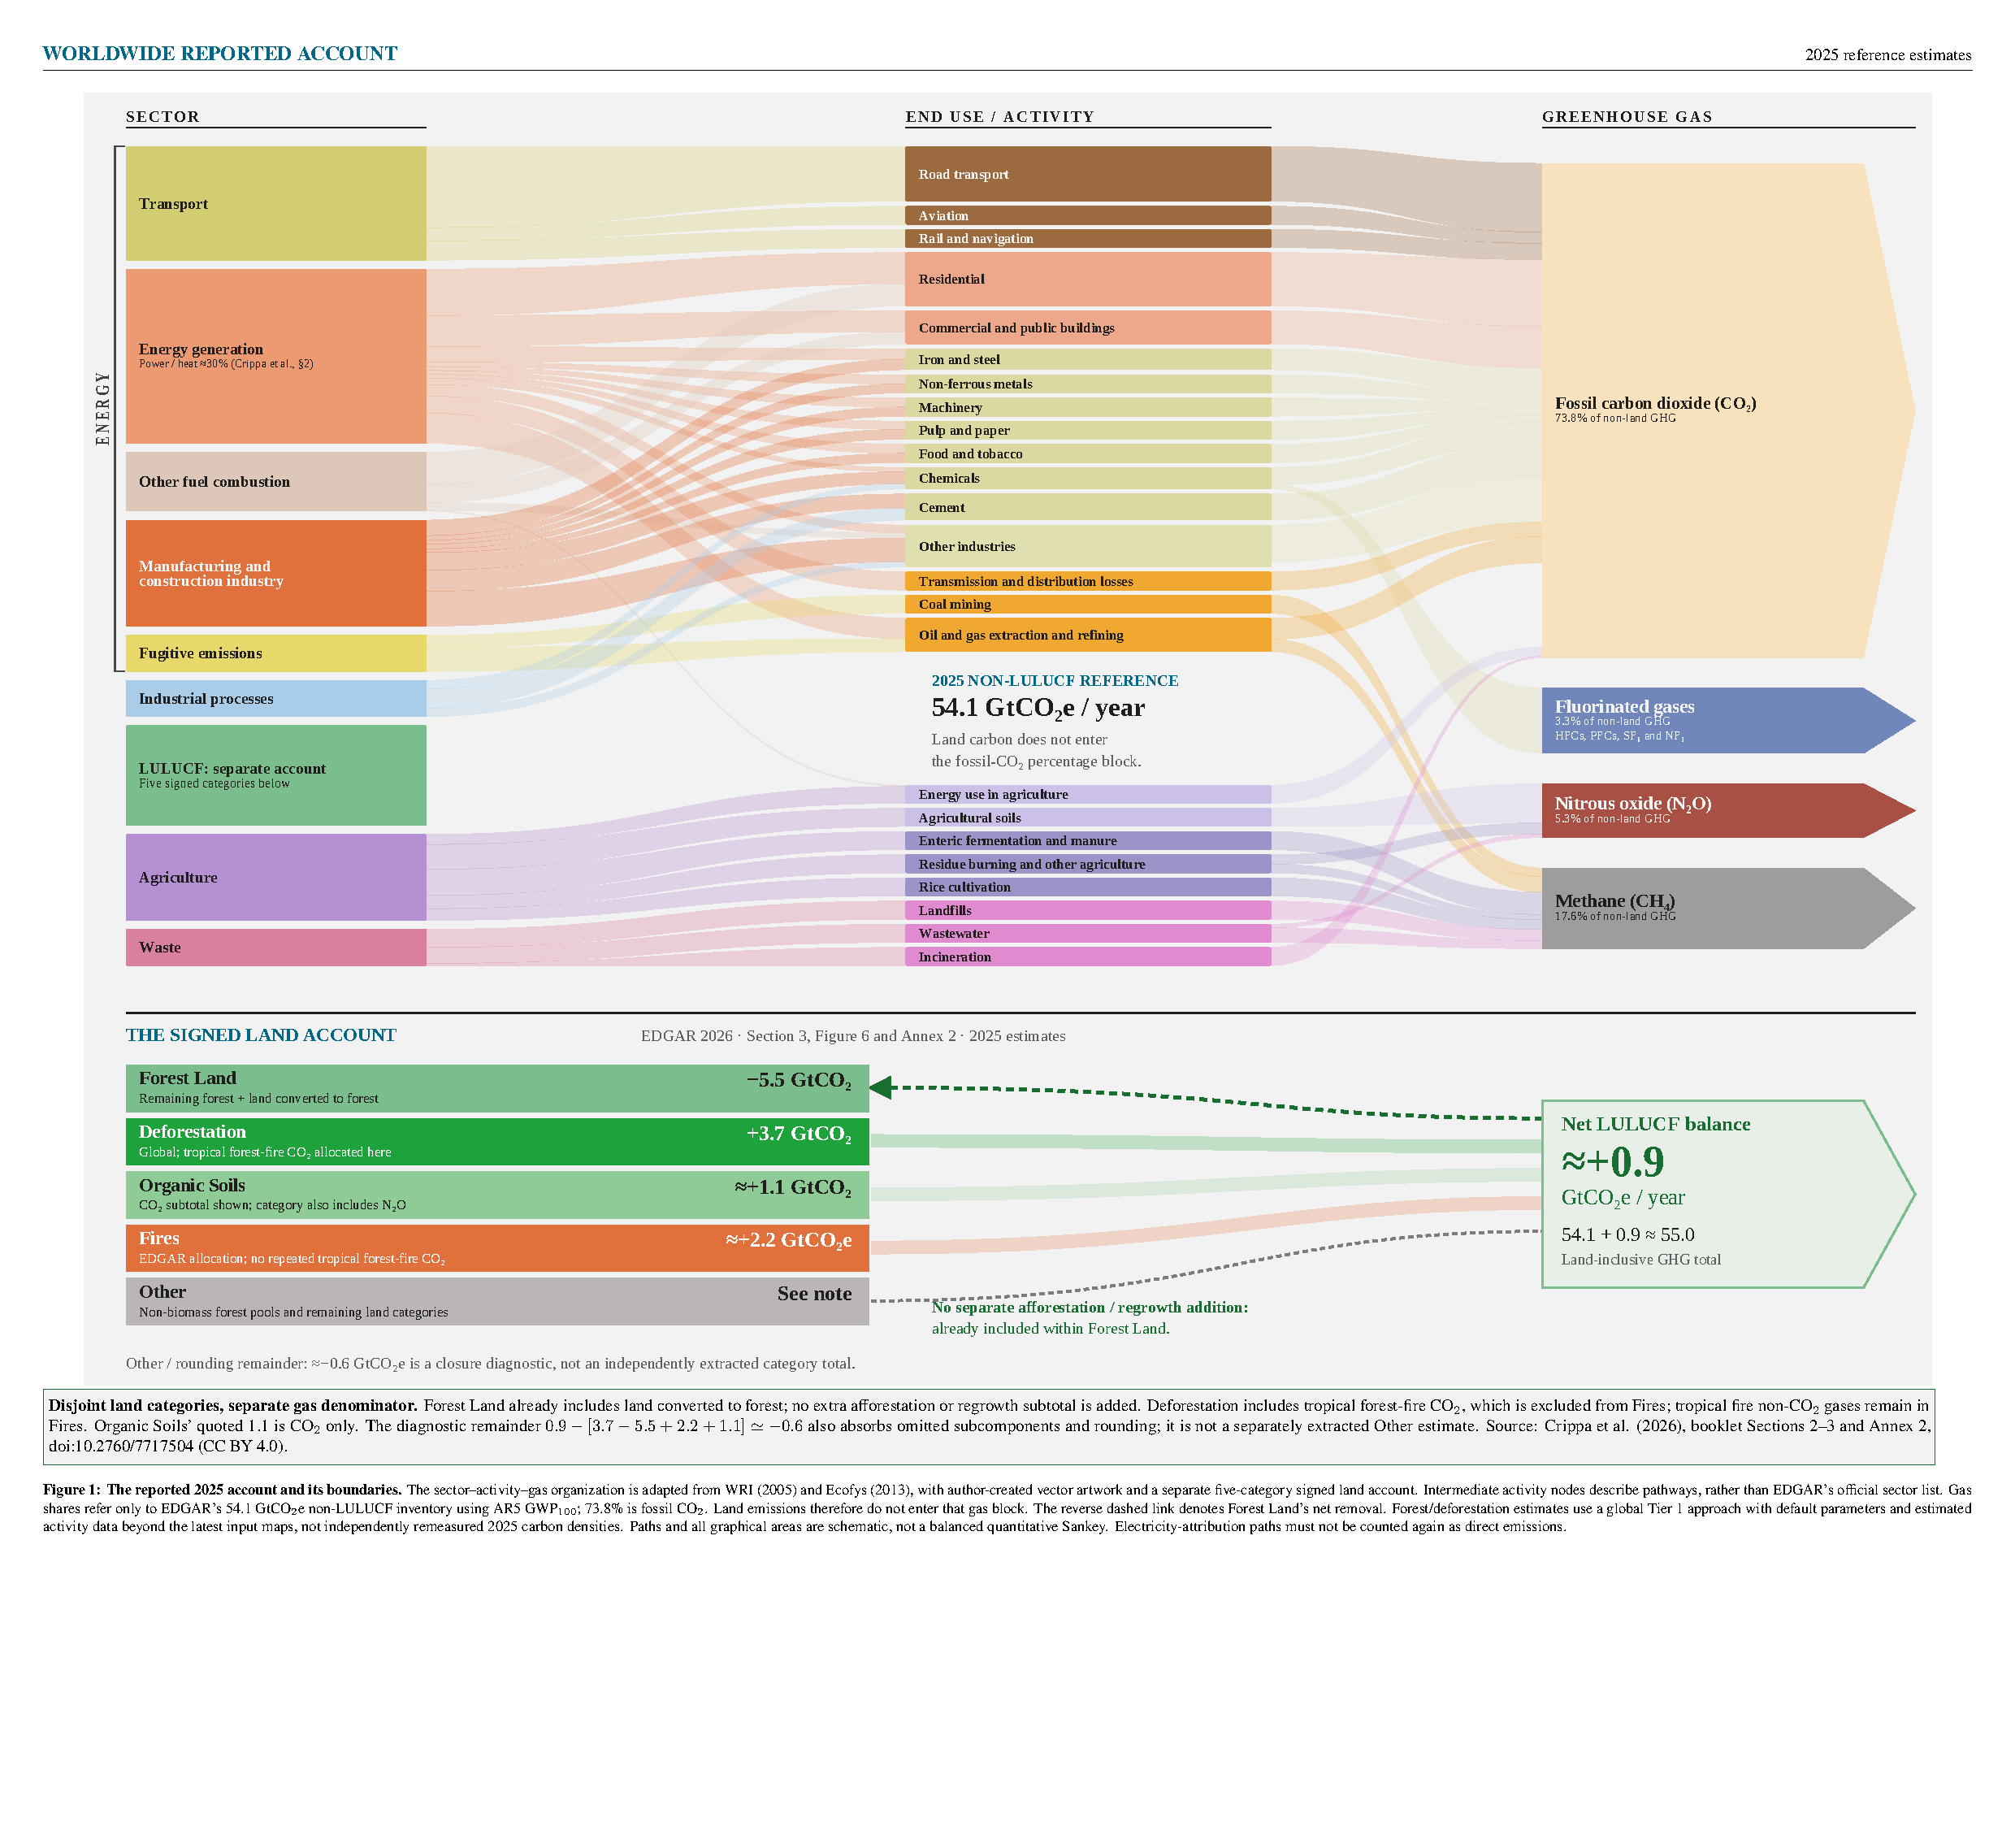
\includepdf[pages=1,fitpaper=true,pagecommand={\thispagestyle{empty}\refstepcounter{figure}\label{fig:reported}}]{figures/figure_plates.pdf}
\includepdf[pages=2,fitpaper=true,pagecommand={\thispagestyle{empty}\refstepcounter{figure}\label{fig:reinterpretation}}]{figures/figure_plates.pdf}
\includepdf[pages=3,fitpaper=true,pagecommand={\thispagestyle{empty}\refstepcounter{figure}\label{fig:physicalclosure}}]{figures/figure_plates.pdf}
\end{document}
